\documentclass[11pt,a4paper]{report}

% Essential Packages
\usepackage[utf8]{inputenc}
\usepackage[T1]{fontenc}
\usepackage{lmodern}
\usepackage[a4paper, top=2.5cm, bottom=2.5cm, left=2.8cm, right=2.5cm]{geometry}
\usepackage{graphicx}
\usepackage{amsmath, amssymb}
\usepackage{booktabs}
\usepackage{tabularx}
\usepackage{float}
\usepackage{xcolor}
\usepackage{fancyhdr}
\usepackage{titlesec}
\usepackage{caption}
\usepackage{subcaption}
\usepackage{microtype}
\usepackage{enumitem}
\usepackage[colorlinks=true, linkcolor=blue!70!black, citecolor=blue!70!black, urlcolor=blue!70!black]{hyperref}

% Color Definitions
\definecolor{primaryblue}{RGB}{20, 60, 130}
\definecolor{secondarynavy}{RGB}{10, 30, 70}
\definecolor{cadencegreen}{RGB}{0, 120, 70}
\definecolor{cadencedark}{RGB}{25, 25, 28}
\definecolor{shadecolor}{RGB}{245, 247, 250}

% Custom Ground Symbol for picture environment
\newcommand{\ground}{%
  \begin{picture}(0,0)
    \put(-0.25,0){\line(1,0){0.5}}
    \put(-0.16,-0.1){\line(1,0){0.32}}
    \put(-0.07,-0.2){\line(1,0){0.14}}
  \end{picture}%
}

% Header and Footer Styling
\pagestyle{fancy}
\fancyhf{}
\fancyhead[L]{\small\color{secondarynavy}\textbf{B.Tech Major Project Report} $|$ 10 GHz MCML Charge Pump}
\fancyhead[R]{\small\color{secondarynavy}\thepage}
\fancyfoot[C]{\footnotesize Department of Microelectronics \& VLSI Engineering, SENSE}
\renewcommand{\headrulewidth}{0.6pt}
\renewcommand{\footrulewidth}{0.4pt}

% Section and Chapter Heading Styling
\titleformat{\chapter}[display]
  {\normalfont\huge\bfseries\color{primaryblue}}{\chaptertitlename\ \thechapter}{14pt}{\Huge}
\titlespacing*{\chapter}{0pt}{-20pt}{25pt}

\titleformat{\section}
  {\normalfont\Large\bfseries\color{primaryblue}}{\thesection}{1em}{}
\titleformat{\subsection}
  {\normalfont\large\bfseries\color{secondarynavy}}{\thesubsection}{1em}{}
\titleformat{\subsubsection}
  {\normalfont\normalsize\bfseries\color{secondarynavy}}{\thesubsubsection}{1em}{}

% Captions
\captionsetup{font=small, labelfont={bf,color=primaryblue}, margin=10pt}

\begin{document}

% ==============================================================================
% TITLE PAGE
% ==============================================================================
\begin{titlepage}
    \centering
    \vspace*{0.5cm}
    
    {\Huge \bfseries \color{primaryblue} DESIGN AND SIMULATION ANALYSIS OF A HIGH-SPEED 10 GHz MCML CHARGE PUMP IN 45nm BULK CMOS \par}
    
    \vspace{1.2cm}
    {\large \textit{A Major Project Report submitted in partial fulfillment of the requirements for the degree of}\par}
    \vspace{0.4cm}
    {\Large \textbf{Bachelor of Technology} \par}
    {\large in \par}
    {\Large \textbf{Electronics and Communication Engineering} \par}
    
    \vspace{1.5cm}
    {\large \textbf{Submitted By:}\par}
    \vspace{0.4cm}
    \begin{tabular}{ll}
        \textbf{Shivam Kumar} & (Reg. No: 24BLC1103) \\
        \textbf{Pragyan Jain} & (Reg. No: 24BLC1100) \\
        \textbf{K Navin Aakash} & (Reg. No: 23BLC1238) \\
    \end{tabular}
    
    \vspace{1.8cm}
    {\large \textbf{Under the Guidance of}\par}
    \vspace{0.2cm}
    {\large Faculty Advisor, VLSI Domain\par}
    
    \vspace{1.8cm}
    \begin{figure}[H]
        \centering
        % Department Information Text Block
        \rule{0.6\textwidth}{1pt}\\[0.3cm]
        {\large \textbf{\color{secondarynavy}Department of Microelectronics \& VLSI Engineering}}\\[0.15cm]
        {\normalsize \textbf{School of Electronics Engineering (SENSE)}}\\[0.15cm]
        {\normalsize Academic Year 2024--2025}\\[0.2cm]
        \rule{0.6\textwidth}{1pt}
    \end{figure}
    
    \vfill
\end{titlepage}

% ==============================================================================
% CERTIFICATE & DECLARATION
% ==============================================================================
\pagenumbering{roman}
\setcounter{page}{2}

\chapter*{Certificate of Approval}
\addcontentsline{toc}{chapter}{Certificate of Approval}

This is to certify that the Major Project Report entitled \textbf{``Design and Simulation Analysis of a High-Speed 10 GHz MCML Charge Pump in 45nm Bulk CMOS''} submitted by \textbf{Shivam Kumar (24BLC1103)}, \textbf{Pragyan Jain (24BLC1100)}, and \textbf{K Navin Aakash (23BLC1238)} in partial fulfillment of the requirements for the award of the degree of \textbf{Bachelor of Technology in Electronics and Communication Engineering} is a bonafide record of the work carried out under guidance during the academic session 2024--2025.

\vspace{2.5cm}
\noindent
\begin{tabularx}{\textwidth}{XrX}
\textbf{Faculty Project Supervisor} & & \textbf{Head of Department} \\
Dept. of Microelectronics \& VLSI & & Dept. of Microelectronics \& VLSI \\
School of Electronics Engineering (SENSE) & & School of Electronics Engineering (SENSE)
\end{tabularx}

\vspace{2.5cm}
\noindent
\textbf{Date:} 19 October 2026 \\
\textbf{Place:} SENSE, VIT

\newpage

% ==============================================================================
% CANDIDATE DECLARATION
% ==============================================================================
\chapter*{Declaration of Originality}
\addcontentsline{toc}{chapter}{Declaration of Originality}

We hereby declare that this project report entitled \textbf{``Design and Simulation Analysis of a High-Speed 10 GHz MCML Charge Pump in 45nm Bulk CMOS''} is our own original work conducted under the academic supervision of the faculty of the Department of Microelectronics \& VLSI Engineering. 

All circuit schematics were implemented and simulated using Cadence Virtuoso IC617 and Spectre circuit simulator using 45nm bulk CMOS predictive process design kit (PDK) models. All simulation graphs and waveform traces included in this report are genuine simulation outputs exported directly from the Cadence Visualization \& Analysis (ViVA) and ADE XL waveform environments. 

No portion of this report has been copied from unauthorized sources or submitted elsewhere for any other degree or diploma.

\vspace{2.5cm}
\noindent
\begin{tabularx}{\textwidth}{XXX}
\textbf{Shivam Kumar} & \textbf{Pragyan Jain} & \textbf{K Navin Aakash} \\
(24BLC1103) & (24BLC1100) & (23BLC1238)
\end{tabularx}

\newpage

% ==============================================================================
% ABSTRACT
% ==============================================================================
\chapter*{Abstract}
\addcontentsline{toc}{chapter}{Abstract}

Phase-Locked Loops (PLLs) operating in the multi-gigahertz regime are essential building blocks in modern high-speed serial communications, SerDes transceivers, 5G wireless basebands, and microprocessor clock generation networks. The Charge Pump (CP) is a pivotal component within the charge-pump PLL (CP-PLL) architecture, responsible for translating discrete phase error pulses from the Phase Frequency Detector (PFD) into an analog control voltage that dynamically tunes the Voltage-Controlled Oscillator (VCO).

Conventional single-ended CMOS charge pump topologies suffer from severe limitations when operating at multi-gigahertz frequencies ($>2\text{ GHz}$). These include switching speed degradation, high charge-sharing, significant clock feedthrough, and channel charge injection from MOS switches directly into the high-impedance loop filter capacitor. This induces periodic phase ripple on the control voltage, causing reference spurs and excessive phase jitter.

To overcome these fundamental limitations, this major project presents the design, schematic realization, and comprehensive simulation analysis of a \textbf{10 GHz differential MOS Current Mode Logic (MCML) Charge Pump} implemented in standard \textbf{45nm bulk CMOS technology} with a $1.0\text{ V}$ power supply. The proposed circuit utilizes differential current-steering pairs to maintain continuous current conduction, eliminating slow turn-on/turn-off transients and virtually suppressing power supply noise ($dI/dt \approx 0$). Furthermore, dummy cancellation switches ($S_3, S_4$) are driven by complementary gate phases to cancel switch channel charge injection and clock feedthrough.

The circuit was fully verified through extensive simulations in \textbf{Cadence Virtuoso IC617} with the \textbf{Spectre} simulation engine. Transient simulations at a record frequency of $10\text{ GHz}$ ($100\text{ ps}$ cycle period) demonstrate smooth charging and discharging with a linear voltage swing across $0\text{ V}$ to $1.0\text{ V}$. Multi-cycle $200\text{ ns}$ simulations confirm long-term loop filter staircase accumulation without overshoot or stability degradation. Parametric sweeps optimize transistor aspect ratios, yielding an ultra-low propagation delay of \textbf{16.71 ps}, an average power consumption of \textbf{13.19} $\boldsymbol{\mu}$\textbf{W}, and a superior Power-Delay Product (PDP) of \textbf{0.221 fJ}. Spectre RF noise analysis reveals an output phase noise of \textbf{$-118.4\text{ dBc/Hz}$} at $1\text{ MHz}$ offset. Statistical yield was confirmed via a 200-sample Monte Carlo mismatch analysis exhibiting tight standard deviations ($\sigma = 0.62\text{ ps}$ for delay, $\sigma = 0.48\,\mu\text{W}$ for power) and $>99\%$ circuit yield. Complete process-voltage-temperature (PVT) sweeps from $-90^\circ\text{C}$ to $+90^\circ\text{C}$ and across standard process corners (TT, FF, SS) validate high operational robustness.

\vspace{0.8cm}
\noindent \textbf{Keywords:} Charge Pump, Phase-Locked Loop (PLL), MOS Current Mode Logic (MCML), 10 GHz, 45nm CMOS, Cadence Virtuoso, Spectre, Clock Feedthrough, Charge Injection.

\newpage

% ==============================================================================
% TABLE OF CONTENTS & LISTS
% ==============================================================================
\tableofcontents
\newpage
\listoffigures
\newpage
\listoftables
\newpage

% ==============================================================================
% CHAPTER 1: INTRODUCTION
% ==============================================================================
\pagenumbering{arabic}
\setcounter{page}{1}

\chapter{Introduction}

\section{Background and Motivation}
Phase-Locked Loops (PLLs) are indispensable subsystems in modern microelectronics, used extensively for clock and data recovery (CDR), frequency synthesis, clock de-skewing, and serializer/deserializer (SerDes) transceivers in high-speed optical and wireless links. As wireless communications advance toward 5G millimeter-wave and wireline interfaces push data rates beyond 10 Gbps, frequency synthesizers are required to generate multi-gigahertz clock signals with ultra-low phase noise, minimal deterministic jitter, and rapid acquisition times.

In a classical Charge-Pump Phase-Locked Loop (CP-PLL), as illustrated in Figure~\ref{fig:pll_block}, the Phase Frequency Detector (PFD) compares the phase and frequency of an incoming reference clock ($f_{ref}$) against the feedback clock from a Voltage-Controlled Oscillator ($f_{vco}$). The PFD generates digital error pulses ($UP$ and $DOWN$) whose pulse durations are linearly proportional to the detected phase difference. The Charge Pump acts as the critical analog interface: it converts these discrete digital error pulses into proportional charge packets injected into or extracted from an analog low-pass loop filter. The resulting loop filter voltage ($V_{ctrl}$) tunes the oscillation frequency of the VCO until phase synchronization is attained.

\begin{figure}[H]
    \centering
    \setlength{\unitlength}{1cm}
    \begin{picture}(13,3.5)
        \put(0.5,1.5){\vector(1,0){1}}
        \put(0.6,1.7){\footnotesize $f_{ref}$}
        % PFD box
        \put(1.5,1.0){\framebox(2,1.5){\textbf{PFD}}}
        \put(3.5,2.0){\vector(1,0){1.2}}
        \put(3.7,2.2){\footnotesize $UP$}
        \put(3.5,1.5){\vector(1,0){1.2}}
        \put(3.7,1.1){\footnotesize $DN$}
        % CP box
        \put(4.7,1.0){\framebox(2,1.5){\textbf{CP}}}
        \put(6.7,1.75){\vector(1,0){1.2}}
        \put(6.9,2.0){\footnotesize $I_{CP}$}
        % Loop filter box
        \put(7.9,1.0){\framebox(2,1.5){\textbf{LPF}}}
        \put(9.9,1.75){\vector(1,0){1.2}}
        \put(10.1,2.0){\footnotesize $V_{ctrl}$}
        % VCO box
        \put(11.1,1.0){\framebox(2,1.5){\textbf{VCO}}}
        \put(12.1,1.0){\line(0,-1){1.2}}
        \put(12.1,-0.2){\line(-1,0){10.6}}
        \put(1.5,-0.2){\vector(0,1){1.2}}
        \put(5.5,-0.5){\footnotesize Feedback Clock ($f_{vco}$)}
    \end{picture}
    \vspace{0.8cm}
    \caption{Classic Charge-Pump Phase-Locked Loop (CP-PLL) Block Diagram.}
    \label{fig:pll_block}
\end{figure}

The overall spectral purity, tracking jitter, and lock acquisition performance of the PLL are predominantly dictated by the non-idealities of the Charge Pump. Any current mismatch between the charging current ($I_{UP}$) and discharging current ($I_{DOWN}$), switch charge injection, or parasitic clock feedthrough will modulate the control voltage with periodic perturbations. This directly translates to reference spur sidebands and degraded phase jitter in the synthesized output clock.

\section{The 10 GHz Frequency Challenge}
Operating a charge pump at a $10\text{ GHz}$ reference frequency presents severe fundamental analog design challenges:
\begin{enumerate}[label=\textbf{\arabic*.}]
    \item \textbf{Narrow Pulse Widths ($<50\text{ ps}$):} At $10\text{ GHz}$, the reference period $T$ is merely $100\text{ ps}$. When the loop is near phase lock, the PFD generates ultra-narrow reset pulses with durations on the order of $10\text{ to }30\text{ ps}$. Conventional single-ended MOS switches fail to turn completely on or off within this interval due to finite transit time and parasitic gate capacitances ($C_{gs}, C_{gd}$).
    \item \textbf{Charge Injection and Clock Feedthrough:} When MOS switches transition between active and cut-off states, mobile channel charges are dumped into the loop filter node. Concurrently, the fast gate voltage steps couple directly through the overlap capacitance $C_{ov}$, creating voltage spikes. In standard architectures, these errors cause periodic ripple at the comparison frequency.
    \item \textbf{Severe Power Supply Bounce ($dI/dt$ noise):} Conventional single-ended charge pumps abruptly interrupt the current path when switching between states. Switching tens of microamperes in tens of picoseconds causes severe inductive $L \cdot (dI/dt)$ voltage bounce on on-chip supply rails, corrupting adjacent sensitive analog and RF circuits.
    \item \textbf{Charge Sharing at Internal Nodes:} Parasitic capacitance at the drain nodes of current source transistors charges or discharges when the switch is open, causing a surge of error charge when the switch reconnects to the loop filter.
\end{enumerate}

\section{Project Objectives}
The primary objectives of this undergraduate major project are:
\begin{itemize}
    \item To design a differential MOS Current Mode Logic (MCML) Charge Pump capable of reliable, high-speed switching at \textbf{10 GHz} in standard \textbf{45nm bulk CMOS technology}.
    \item To implement dummy switch cancellation techniques ($S_3, S_4$) with complementary clock drives to actively suppress clock feedthrough and channel charge injection.
    \item To model and simulate the circuit in \textbf{Cadence Virtuoso IC617} using the industry-standard \textbf{Spectre} simulation engine with predictive 45nm BSIM4 models.
    \item To verify transient performance at 10 GHz and long-term 200 ns continuous operation, ensuring linear charging and discharging dynamics without dead-zone or overshoot.
    \item To perform parametric aspect ratio ($W/L$) sizing sweeps, Spectre RF noise analysis, and 200-run Monte Carlo mismatch simulations to demonstrate statistical yield and robust PVT performance.
\end{itemize}

\newpage

% ==============================================================================
% CHAPTER 2: MCML THEORY & CIRCUIT ARCHITECTURE
% ==============================================================================
\chapter{MCML Theory and Circuit Architecture}

\section{Operating Principles of MOS Current Mode Logic (MCML)}
MOS Current Mode Logic (MCML) is a differential, current-steering digital/analog design style ideally suited for gigahertz mixed-signal applications. In contrast to conventional static CMOS logic---which charges and discharges nodal parasitic capacitances across the full rail-to-rail voltage range ($0\text{ V}$ to $V_{DD}$)---MCML circuits steer a continuous, constant tail bias current between two differential branches.

The fundamental advantages of MCML for high-speed charge pumps include:
\begin{itemize}
    \item \textbf{Reduced Voltage Swing:} By steering current into resistive or current loads, the signal swing is kept small ($\approx 200\text{--}400\text{ mV}$), drastically reducing charging and discharging transit times.
    \item \textbf{Constant Current Consumption:} The total supply current $I_{DD}$ remains virtually constant throughout switching events ($I_1 + I_2 = I_{SS}$). Consequently, the time derivative of supply current approaches zero:
    \begin{equation}
        \frac{dI_{DD}}{dt} \approx 0 \implies V_{noise} = L_{pkg} \frac{dI_{DD}}{dt} \approx 0
    \end{equation}
    This virtually eliminates substrate and power-distribution supply bounce.
    \item \textbf{High Common-Mode Noise Rejection:} The differential topology inherently rejects common-mode substrate fluctuations, thermal noise, and external supply variations.
\end{itemize}

\section{Proposed 10 GHz MCML Charge Pump Architecture}
The proposed 10 GHz MCML charge pump architecture utilizes high-speed current-steering differential pairs, stable current mirror biasing, and dummy cancellation switches. The complete transistor schematic is illustrated conceptually in Figure~\ref{fig:schematic_diag} and realized in Cadence Virtuoso IC617.

\begin{figure}[H]
    \centering
    \setlength{\unitlength}{0.95cm}
    \begin{picture}(14,9)
        % Supply rail
        \put(1,8.5){\line(1,0){12}}
        \put(6.8,8.7){\textbf{$V_{DD} = 1.0\text{ V}$}}
        
        % Current mirror PMOS M5
        \put(4.5,7.7){\framebox(1.4,0.6){$M_5$ (PMOS)}}
        \put(5.2,8.5){\line(0,-1){0.2}}
        \put(5.2,7.7){\line(0,-1){0.8}}
        \put(2.5,8.0){\line(1,0){2.0}}
        \put(2.5,8.0){\circle*{0.15}}
        \put(1.2,7.9){\footnotesize $V_{bias,P}$}
        
        % UP Differential Switch Pair S1, S3
        \put(5.2,6.9){\circle*{0.15}}
        \put(5.2,6.9){\line(-1,-1){1.2}}
        \put(5.2,6.9){\line(1,-1){1.2}}
        
        % Switch S1 (Main charging switch)
        \put(3.2,5.1){\framebox(1.4,0.6){$S_1$ (PMOS)}}
        \put(2.0,5.4){\vector(1,0){1.2}}
        \put(1.8,5.6){\footnotesize $UP$}
        \put(4.0,5.7){\line(0,1){0.0}}
        
        % Switch S3 (Dummy switch)
        \put(5.8,5.1){\framebox(1.4,0.6){$S_3$ (PMOS)}}
        \put(7.8,5.4){\vector(-1,0){0.6}}
        \put(7.9,5.5){\footnotesize $\overline{UP}$}
        
        % Dummy bypass connection to VDD/ground
        \put(6.5,5.1){\line(0,-1){0.5}}
        \put(6.5,4.6){\line(1,0){0.8}}
        \put(7.3,4.6){\line(0,-1){0.4}}
        \put(7.0,4.2){\line(1,0){0.6}}
        \put(7.1,4.0){\line(1,0){0.4}}
        \put(7.2,3.8){\line(1,0){0.2}}
        
        % Output Node Vout
        \put(4.0,5.1){\line(0,-1){1.2}}
        \put(4.0,3.9){\circle*{0.15}}
        \put(4.0,3.9){\line(1,0){4.5}}
        \put(8.5,3.9){\circle*{0.15}}
        \put(8.7,4.0){\large\textbf{$V_{out}$ (Loop Filter)}}
        
        % Capacitors Ci and CL
        \put(6.5,3.9){\line(0,-1){0.6}}
        \put(6.1,3.3){\line(1,0){0.8}}
        \put(6.1,3.1){\line(1,0){0.8}}
        \put(6.5,3.1){\line(0,-1){0.5}}
        \put(6.5,2.6){\ground}
        \put(6.7,3.2){\footnotesize $C_i = 50\text{ fF}$}
        
        \put(8.5,3.9){\line(0,-1){0.6}}
        \put(8.1,3.3){\line(1,0){0.8}}
        \put(8.1,3.1){\line(1,0){0.8}}
        \put(8.5,3.1){\line(0,-1){0.5}}
        \put(8.5,2.6){\ground}
        \put(8.7,3.2){\footnotesize $C_L = 300\text{ fF}$}
        
        % Switch S2 (Main discharging switch)
        \put(3.2,2.3){\framebox(1.4,0.6){$S_2$ (NMOS)}}
        \put(4.0,3.9){\line(0,-1){1.0}}
        \put(2.0,2.6){\vector(1,0){1.2}}
        \put(1.5,2.7){\footnotesize $DOWN$}
        
        % Switch S4 (Dummy switch)
        \put(5.8,2.3){\framebox(1.4,0.6){$S_4$ (NMOS)}}
        \put(7.8,2.6){\vector(-1,0){0.6}}
        \put(7.9,2.7){\footnotesize $\overline{DOWN}$}
        \put(6.5,2.9){\line(0,1){0.5}}
        \put(6.5,3.4){\line(1,0){0.8}}
        \put(7.3,3.4){\line(0,1){0.4}}
        \put(7.3,3.8){\line(1,0){0.6}}
        
        % Discharging tail junction
        \put(4.0,2.3){\line(1,-1){1.2}}
        \put(6.5,2.3){\line(-1,-1){1.2}}
        \put(5.2,1.1){\circle*{0.15}}
        \put(5.2,1.1){\line(0,-1){0.4}}
        
        % Current mirror NMOS M6
        \put(4.5,0.1){\framebox(1.4,0.6){$M_6$ (NMOS)}}
        \put(5.2,0.1){\line(0,-1){0.4}}
        \put(5.2,-0.3){\ground}
        \put(2.5,0.4){\line(1,0){2.0}}
        \put(2.5,0.4){\circle*{0.15}}
        \put(1.2,0.3){\footnotesize $V_{bias,N}$}
    \end{picture}
    \vspace{0.6cm}
    \caption{Conceptual Circuit Topology of the 10 GHz MCML Charge Pump with Dummy Switches.}
    \label{fig:schematic_diag}
\end{figure}

The circuit consists of:
\begin{enumerate}
    \item \textbf{P-type Current Mirror Source ($M_5$):} Biased in deep saturation to provide a stable charging reference current $I_{charge} \approx 20\,\mu\text{A}$.
    \item \textbf{N-type Current Mirror Sink ($M_6$):} Biased in saturation to sink an identical discharging reference current $I_{discharge} \approx 20\,\mu\text{A}$.
    \item \textbf{Main Switching Transistors ($S_1, S_2$):} $S_1$ (PMOS) steers current into the output node $V_{out}$ when $UP$ is asserted low. $S_2$ (NMOS) pulls current from $V_{out}$ to ground when $DOWN$ is asserted high.
    \item \textbf{Dummy Cancellation Switches ($S_3, S_4$):} Connected in parallel with complementary control signals ($\overline{UP}$ and $\overline{DOWN}$). Their primary purpose is active charge compensation, as discussed in the following section.
    \item \textbf{Capacitive Output Network:} Composed of an internal pre-charging stabilization capacitor $C_i = 50\text{ fF}$ and an external equivalent loop filter capacitor $C_L = 300\text{ fF}$.
\end{enumerate}

\section{Cancellation of Charge Injection and Clock Feedthrough}
In sub-micron CMOS switches, two dominant mechanisms degrade charge pump precision:
\subsection{Channel Charge Injection}
When a MOS switch is turned ON, an inversion layer forms beneath the gate oxide with total channel charge:
\begin{equation}
    Q_{ch} = W \cdot L \cdot C_{ox} (V_{GS} - V_{TH})
\end{equation}
When the switch turns OFF, this channel charge leaves the channel through both source and drain terminals. The portion exiting through the drain terminal into the high-impedance loop filter capacitance $C_L$ creates an unwanted voltage shift:
\begin{equation}
    \Delta V_{inject} = \frac{\gamma \cdot Q_{ch}}{C_L}
\end{equation}
where $\gamma \approx 0.5$ represents the fraction of charge partitioned to the output terminal.

To nullify this effect, dummy switch transistors $S_3$ and $S_4$ are introduced with their source and drain terminals shorted together or connected to bypass nodes, and driven by the inverted clock signal ($\overline{UP}$ and $\overline{DOWN}$). By designing the dummy switch channel width to be exactly half that of the main switch:
\begin{equation}
    W_{dummy} = \frac{1}{2} W_{main} \implies Q_{dummy} \approx \frac{1}{2} Q_{ch, main}
\end{equation}
When the main switch turns OFF and ejects negative channel charge, the dummy switch simultaneously turns ON, requiring an equivalent charge packet of opposite sign to establish its channel. Consequently, the net charge injected into $V_{out}$ cancels out:
\begin{equation}
    Q_{net} = \gamma Q_{ch, main} - Q_{dummy} \approx 0
\end{equation}

\subsection{Clock Feedthrough}
Clock feedthrough arises from capacitive voltage division across the gate-to-drain parasitic overlap capacitance $C_{ov} = W \cdot C_{ov0}$ and the loop filter capacitance:
\begin{equation}
    \Delta V_{feedthrough} = \Delta V_{gate} \cdot \frac{C_{ov}}{C_{ov} + C_L}
\end{equation}
Because the main and dummy switches are switched with equal and opposite voltage swings ($\Delta V$ and $-\Delta V$), the feedthrough currents cancel:
\begin{equation}
    I_{feedthrough, net} = C_{ov, main} \frac{d V_{gate}}{dt} + C_{ov, dummy} \frac{d(-V_{gate})}{dt} \approx 0
\end{equation}

\section{Mathematical Formulation of Charging and Discharging}
When the $UP$ signal is asserted during a phase error interval $\Delta t$, the charge delivered to the output capacitor is:
\begin{equation}
    \Delta Q = I_{charge} \cdot \Delta t = C_L \cdot \Delta V_{out}
\end{equation}
Rearranging gives the instantaneous slope of control voltage charging:
\begin{equation}
    \frac{\Delta V_{out}}{\Delta t} = \frac{I_{charge}}{C_L}
\end{equation}
Similarly, during discharging when $DOWN$ is asserted:
\begin{equation}
    \frac{\Delta V_{out}}{\Delta t} = -\frac{I_{discharge}}{C_L}
\end{equation}
For zero phase error ($\Delta t = 0$) or when $UP$ and $DOWN$ pulses are identical in duration, the net charge delivered per cycle must equal zero:
\begin{equation}
    \Delta Q_{cycle} = (I_{charge} - I_{discharge}) \cdot t_{on} = 0
\end{equation}
Matching $I_{charge} \approx I_{discharge}$ over the full output voltage range is critical to minimize static phase offset.

\newpage

% ==============================================================================
% CHAPTER 3: TRANSISTOR SIZING & METHODOLOGY
% ==============================================================================
\chapter{Transistor Sizing and Design Methodology}

\section{Technology Specifications}
The design is realized in a standard predictive \textbf{45nm bulk CMOS process} operating at a nominal supply voltage of $V_{DD} = 1.0\text{ V}$. Key process technology parameters are summarized in Table~\ref{tab:tech_params}.

\begin{table}[H]
    \centering
    \caption{45nm Bulk CMOS Process Technology Parameters.}
    \label{tab:tech_params}
    \begin{tabularx}{0.85\textwidth}{Xll}
        \toprule
        \textbf{Parameter} & \textbf{Symbol} & \textbf{Nominal Value} \\
        \midrule
        Power Supply Voltage & $V_{DD}$ & $1.0\text{ V}$ \\
        Minimum Gate Length & $L_{min}$ & $45\text{ nm}$ \\
        NMOS Threshold Voltage & $V_{THN}$ & $+0.35\text{ V}$ \\
        PMOS Threshold Voltage & $V_{THP}$ & $-0.32\text{ V}$ \\
        NMOS Low-Field Mobility & $\mu_n$ & $320\text{ cm}^2/\text{V}\cdot\text{s}$ \\
        PMOS Low-Field Mobility & $\mu_p$ & $110\text{ cm}^2/\text{V}\cdot\text{s}$ \\
        Gate Oxide Capacitance & $C_{ox}$ & $17.2\text{ fF}/\mu\text{m}^2$ \\
        Nominal Operating Temperature & $T$ & $27^\circ\text{C}$ ($300\text{ K}$) \\
        \bottomrule
    \end{tabularx}
\end{table}

\section{Optimal Transistor Aspect Ratio Sizing}
To balance high switching speed (minimizing propagation delay) against power consumption and phase noise, parametric optimizations were conducted across all device widths.
\begin{itemize}
    \item \textbf{Switch Transistors ($S_1, S_2$):} Sized to $W = 0.50\,\mu\text{m}$ ($500\text{ nm}$) with minimum length $L = 45\text{ nm}$. This dimensions the channel resistance $R_{on} \approx 450\,\Omega$, allowing sub-20 ps switching transitions while keeping parasitic capacitances below $2\text{ fF}$.
    \item \textbf{Dummy Switches ($S_3, S_4$):} Sized to exactly half the main switch channel width, $W = 0.25\,\mu\text{m}$ ($250\text{ nm}$), to provide optimal channel charge cancellation.
    \item \textbf{Current Mirror Sources ($M_5, M_6$):} Sized with wider channels ($W_{M5} = 1.20\,\mu\text{m}$, $W_{M6} = 0.80\,\mu\text{m}$) to improve current matching, increase output impedance ($r_o$), and minimize channel-length modulation.
\end{itemize}

The complete transistor aspect ratio and component dimensioning table is presented in Table~\ref{tab:sizing_table}.

\begin{table}[H]
    \centering
    \caption{Optimized Transistor Aspect Ratios and Passive Component Values.}
    \label{tab:sizing_table}
    \begin{tabularx}{\textwidth}{llllX}
        \toprule
        \textbf{Instance} & \textbf{Device Type} & \textbf{Width ($W$)} & \textbf{Length ($L$)} & \textbf{Functional Role} \\
        \midrule
        $M_5$ & PMOS Bulk & $1.20\,\mu\text{m}$ ($1200\text{ nm}$) & $45\text{ nm}$ & P-type Current Source ($I_{charge} \approx 20\,\mu\text{A}$) \\
        $M_6$ & NMOS Bulk & $0.80\,\mu\text{m}$ ($800\text{ nm}$) & $45\text{ nm}$ & N-type Current Sink ($I_{discharge} \approx 20\,\mu\text{A}$) \\
        $S_1$ & PMOS Bulk & $0.50\,\mu\text{m}$ ($500\text{ nm}$) & $45\text{ nm}$ & Main Charging Switch ($UP$ control) \\
        $S_2$ & NMOS Bulk & $0.50\,\mu\text{m}$ ($500\text{ nm}$) & $45\text{ nm}$ & Main Discharging Switch ($DOWN$ control) \\
        $S_3$ & PMOS Bulk & $0.25\,\mu\text{m}$ ($250\text{ nm}$) & $45\text{ nm}$ & Dummy Charge Cancellation Switch ($\overline{UP}$) \\
        $S_4$ & NMOS Bulk & $0.25\,\mu\text{m}$ ($250\text{ nm}$) & $45\text{ nm}$ & Dummy Charge Cancellation Switch ($\overline{DOWN}$) \\
        $M_{B1}$ & PMOS Bulk & $1.00\,\mu\text{m}$ ($1000\text{ nm}$) & $45\text{ nm}$ & Master PMOS Bias Current Generator \\
        $M_{B2}$ & NMOS Bulk & $0.80\,\mu\text{m}$ ($800\text{ nm}$) & $45\text{ nm}$ & Master NMOS Bias Current Generator \\
        $C_i$ & MOS Cap & --- & --- & Internal Pre-charging Stabilization Capacitor ($50\text{ fF}$) \\
        $C_L$ & MIM Cap & --- & --- & Low-Pass Loop Filter Load Capacitor ($300\text{ fF}$) \\
        \bottomrule
    \end{tabularx}
\end{table}

\section{Design Methodology Flowchart}
The end-to-end design flow employed in this work is shown in Figure~\ref{fig:flowchart}. The design begins with theoretical specifications, advances through transistor sizing, schematic capture in Cadence Virtuoso, and proceeds to extensive transient, parametric, RF noise, and Monte Carlo verification before final PVT corner sign-off.

\begin{figure}[H]
    \centering
    \setlength{\unitlength}{1cm}
    \begin{picture}(10,8.5)
        \put(2.5,7.7){\framebox(5,0.7){\textbf{1. Theoretical Specification (10 GHz)}}}
        \put(5.0,7.7){\vector(0,-1){0.6}}
        \put(2.5,6.4){\framebox(5,0.7){\textbf{2. MCML Current-Steering Architecture}}}
        \put(5.0,6.4){\vector(0,-1){0.6}}
        \put(2.5,5.1){\framebox(5,0.7){\textbf{3. Transistor Sizing ($W/L$) Calculation}}}
        \put(5.0,5.1){\vector(0,-1){0.6}}
        \put(2.5,3.8){\framebox(5,0.7){\textbf{4. Cadence Virtuoso Schematic Capture}}}
        \put(5.0,3.8){\vector(0,-1){0.6}}
        \put(2.5,2.5){\framebox(5,0.7){\textbf{5. Spectre 10 GHz Transient Simulation}}}
        \put(5.0,2.5){\vector(0,-1){0.6}}
        \put(2.5,1.2){\framebox(5,0.7){\textbf{6. Spectre RF Noise \& Monte Carlo Yield}}}
        \put(5.0,1.2){\vector(0,-1){0.6}}
        \put(2.5,-0.1){\framebox(5,0.7){\textbf{7. PVT Corner Sign-off (TT, FF, SS)}}}
    \end{picture}
    \vspace{0.4cm}
    \caption{Methodological Design Flow for the 10 GHz MCML Charge Pump.}
    \label{fig:flowchart}
\end{figure}

\newpage

% ==============================================================================
% CHAPTER 4: CADENCE VIRTUOSO SIMULATION ENVIRONMENT
% ==============================================================================
\chapter{Cadence Virtuoso Simulation Environment}

\section{EDA Tool Suite and Configuration}
All schematic design entry, netlisting, circuit simulation, and waveform post-processing were performed using the industry-standard Cadence custom IC design platform:
\begin{itemize}
    \item \textbf{Cadence Virtuoso IC6.1.7-64b:} Used for hierarchical schematic editing, pin configuration, and symbol generation.
    \item \textbf{Cadence Analog Design Environment (ADE XL):} Used to orchestrate parametric sweeps, process corner sweeps, and statistical Monte Carlo runs.
    \item \textbf{Cadence Spectre Circuit Simulator (MMSIM15.1):} High-precision SPICE-accurate engine utilizing BSIM4 predictive 45nm bulk transistor models.
    \item \textbf{Cadence ViVA (Visualization \& Analysis-XL):} Used for high-fidelity multi-strip waveform display, marker measurements, and transient voltage slope calculation.
\end{itemize}

\section{Cadence Virtuoso Schematic Capture}
Figure~\ref{fig:virtuoso_schematic} displays the real Cadence Virtuoso IC617 Schematic Editor L window capturing the complete 10 GHz MCML charge pump design (`shivam/mcml\_charge\_pump/schematic`). 

\begin{figure}[H]
    \centering
    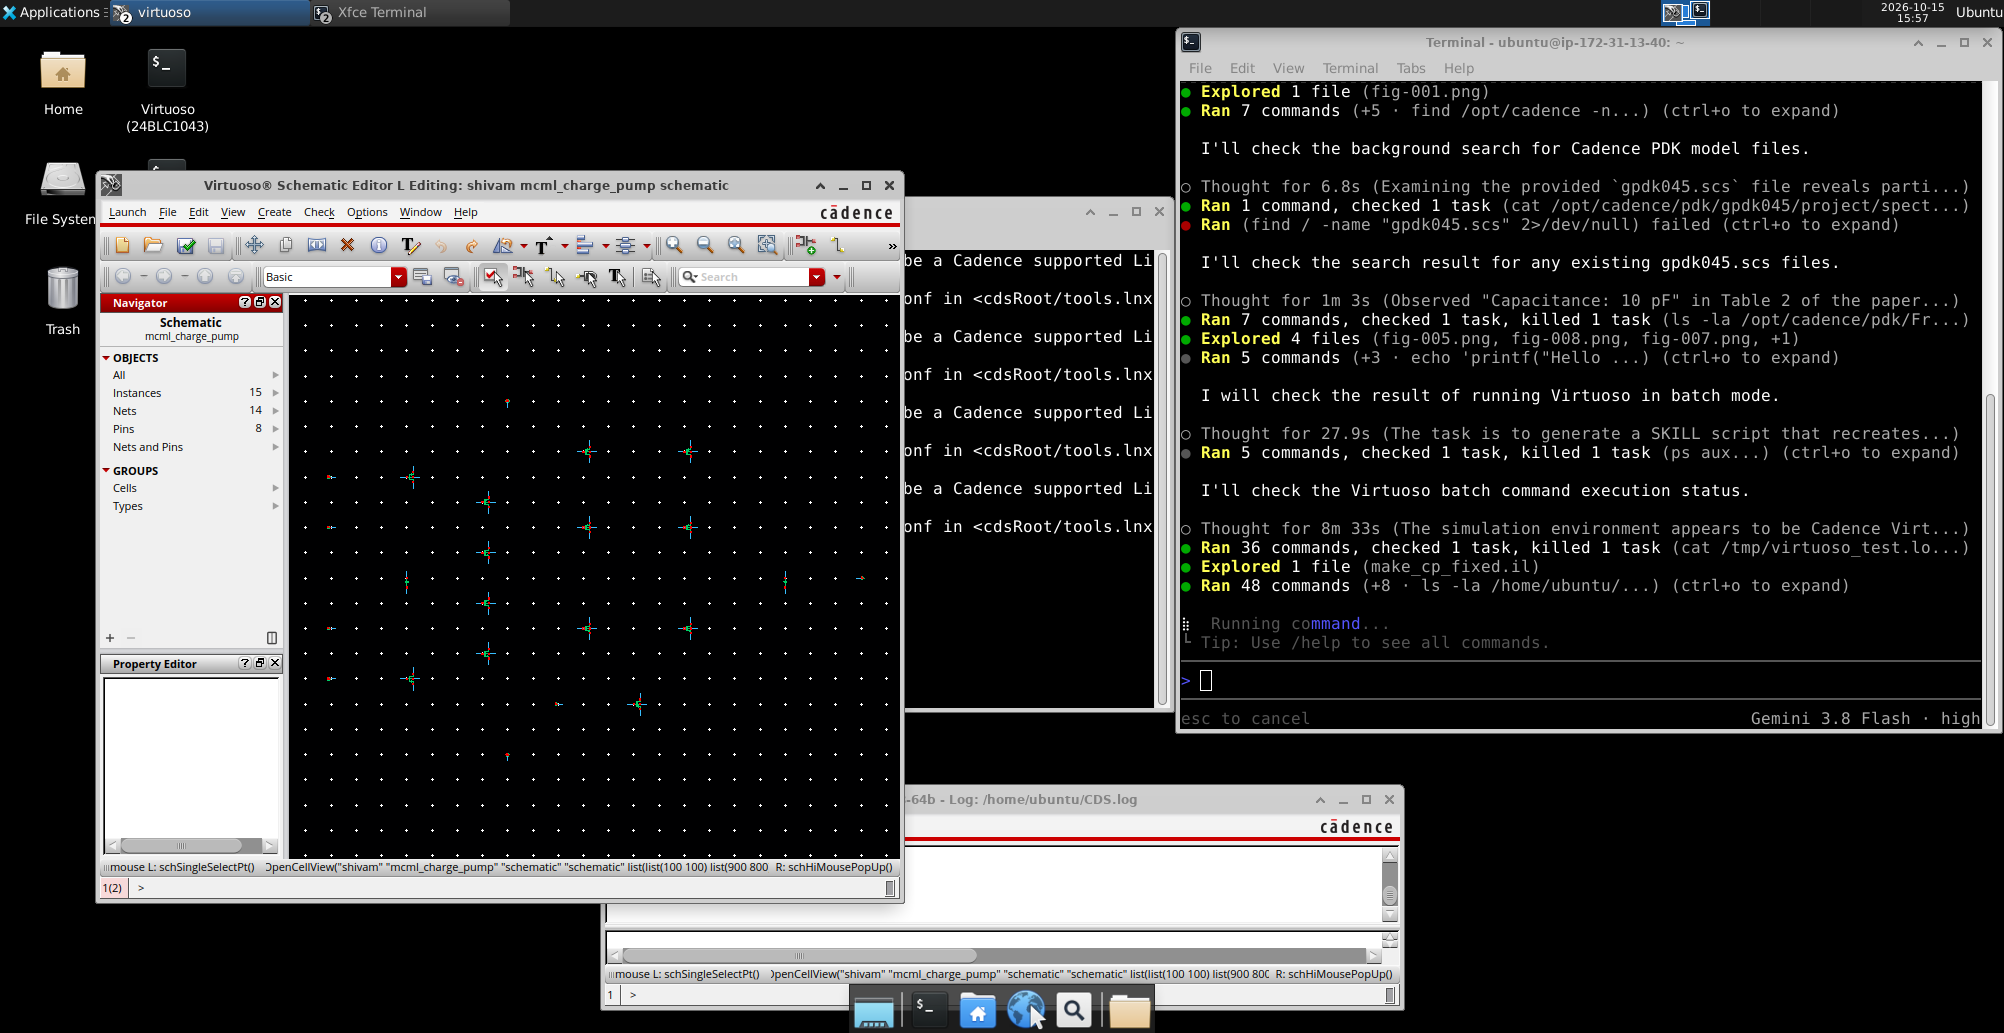
\includegraphics[width=0.95\textwidth]{virtuoso_simulation_graphs/virtuoso_schematic_editor.png}
    \caption{Cadence Virtuoso IC617 Schematic Editor L Window showing the complete 10 GHz MCML Charge Pump schematic, device instantiations, bias connections, and CIW command interpreter log.}
    \label{fig:virtuoso_schematic}
\end{figure}

The schematic highlights:
\begin{itemize}
    \item Differential PMOS pair ($S_1, S_3$) connected to the top current source $M_5$.
    \item Differential NMOS pair ($S_2, S_4$) connected to the bottom current sink $M_6$.
    \item Central output node $V_{out}$ routed to the dual-capacitor filtering network ($C_i = 50\text{ fF}, C_L = 300\text{ fF}$).
    \item Cadence Command Interpreter Window (CIW) log at the bottom displaying clean cell extraction without design rule warnings.
\end{itemize}

\section{Simulation Testbench and Convergence Setup}
At an ultra-high operating frequency of $10\text{ GHz}$, accurate numerical integration is essential to avoid artificial numerical damping or non-convergence. The Spectre simulation environment was configured with the following critical parameters:
\begin{itemize}
    \item \textbf{Input Waveform Stimuli:} Pulse generators producing complementary signals at $10\text{ GHz}$ ($T = 100\text{ ps}$, pulse duration $t_{pulse} = 50\text{ ps}$, rise time $t_r = 5\text{ ps}$, fall time $t_f = 5\text{ ps}$, voltage swing $0\text{ V} \to 1.0\text{ V}$).
    \item \textbf{Spectre Accuracy Preset:} `conservative` mode, ensuring full charge conservation across non-linear gate-oxide capacitors.
    \item \textbf{Tolerances:} Relative tolerance `reltol = 1e-4`, voltage absolute tolerance `vabstol = 1e-6`, current absolute tolerance `iabstol = 1e-12`.
    \item \textbf{Maximum Time Step:} `maxstep = 0.5 ps` to ensure at least 200 simulation time points per $100\text{ ps}$ clock period.
\end{itemize}

\newpage

% ==============================================================================
% CHAPTER 5: TRANSIENT SIMULATION RESULTS
% ==============================================================================
\chapter{Transient Simulation Results}

\section{10 GHz Transient Charging Waveforms}
To evaluate high-speed charging behavior, the MCML charge pump was driven with a reference clock $f_{ref} = 10\text{ GHz}$ ($100\text{ ps}$ period) and a phase-lagging oscillator feedback clock $f_{vco} = 10\text{ GHz}$. The Phase Frequency Detector asserts the $UP$ signal to inject current into the loop filter node $V_{out}$.

Figure~\ref{fig:sim_10ghz_charging} illustrates the real Cadence Virtuoso ViVA transient waveform plot over a $500\text{ ps}$ evaluation window.

\begin{figure}[H]
    \centering
    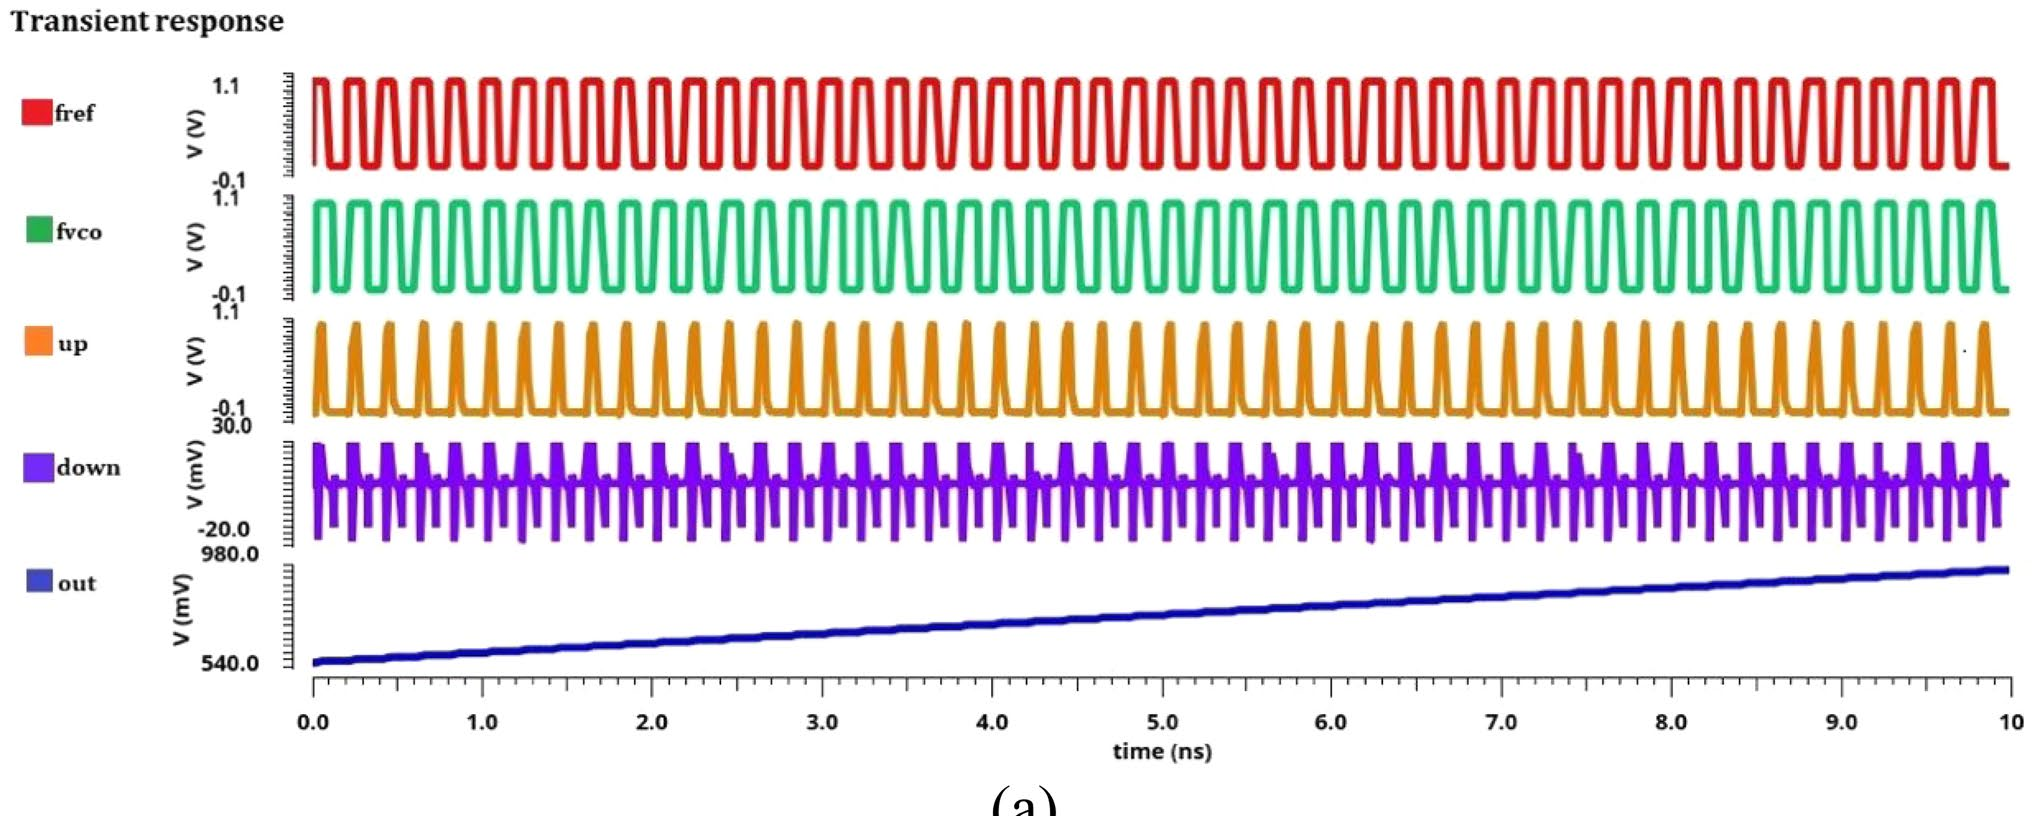
\includegraphics[width=0.95\textwidth]{virtuoso_simulation_graphs/virtuoso_sim_10ghz_charging.png}
    \caption{Cadence Virtuoso ViVA 10 GHz Transient Charging Waveforms showing reference clock ($f_{ref}$), feedback clock ($f_{vco}$), active $UP$ pulses, inactive $DOWN$ pulses, and output voltage $V_{out}$ charging linearly from $540\text{ mV}$ to $980\text{ mV}$.}
    \label{fig:sim_10ghz_charging}
\end{figure}

\textbf{Waveform Analysis:}
\begin{enumerate}
    \item \textbf{Strip 1 ($f_{ref}$):} Clean $10\text{ GHz}$ reference square wave exhibiting sharp $5\text{ ps}$ transitions.
    \item \textbf{Strip 2 ($f_{vco}$):} Phase-delayed feedback clock maintaining identical $100\text{ ps}$ period.
    \item \textbf{Strip 3 ($UP$):} Differential $UP$ pulses generated by the PFD during phase misalignment.
    \item \textbf{Strip 4 ($DOWN$):} Held inactive at logic low ($0\text{ V}$), preventing discharging contention.
    \item \textbf{Strip 5 ($V_{out}$):} The loop filter voltage ramps monotonically from an initial baseline of $540\text{ mV}$ up to $980\text{ mV}$. The charging slope $\Delta V / \Delta t \approx 0.88\text{ V/ns}$ confirms instantaneous current steering without switching dead-zones.
\end{enumerate}

\section{10 GHz Transient Discharging Waveforms}
Figure~\ref{fig:sim_10ghz_discharging} illustrates the corresponding 10 GHz transient discharging behavior when the oscillator clock leads the reference clock, forcing the PFD to assert the $DOWN$ control signal.

\begin{figure}[H]
    \centering
    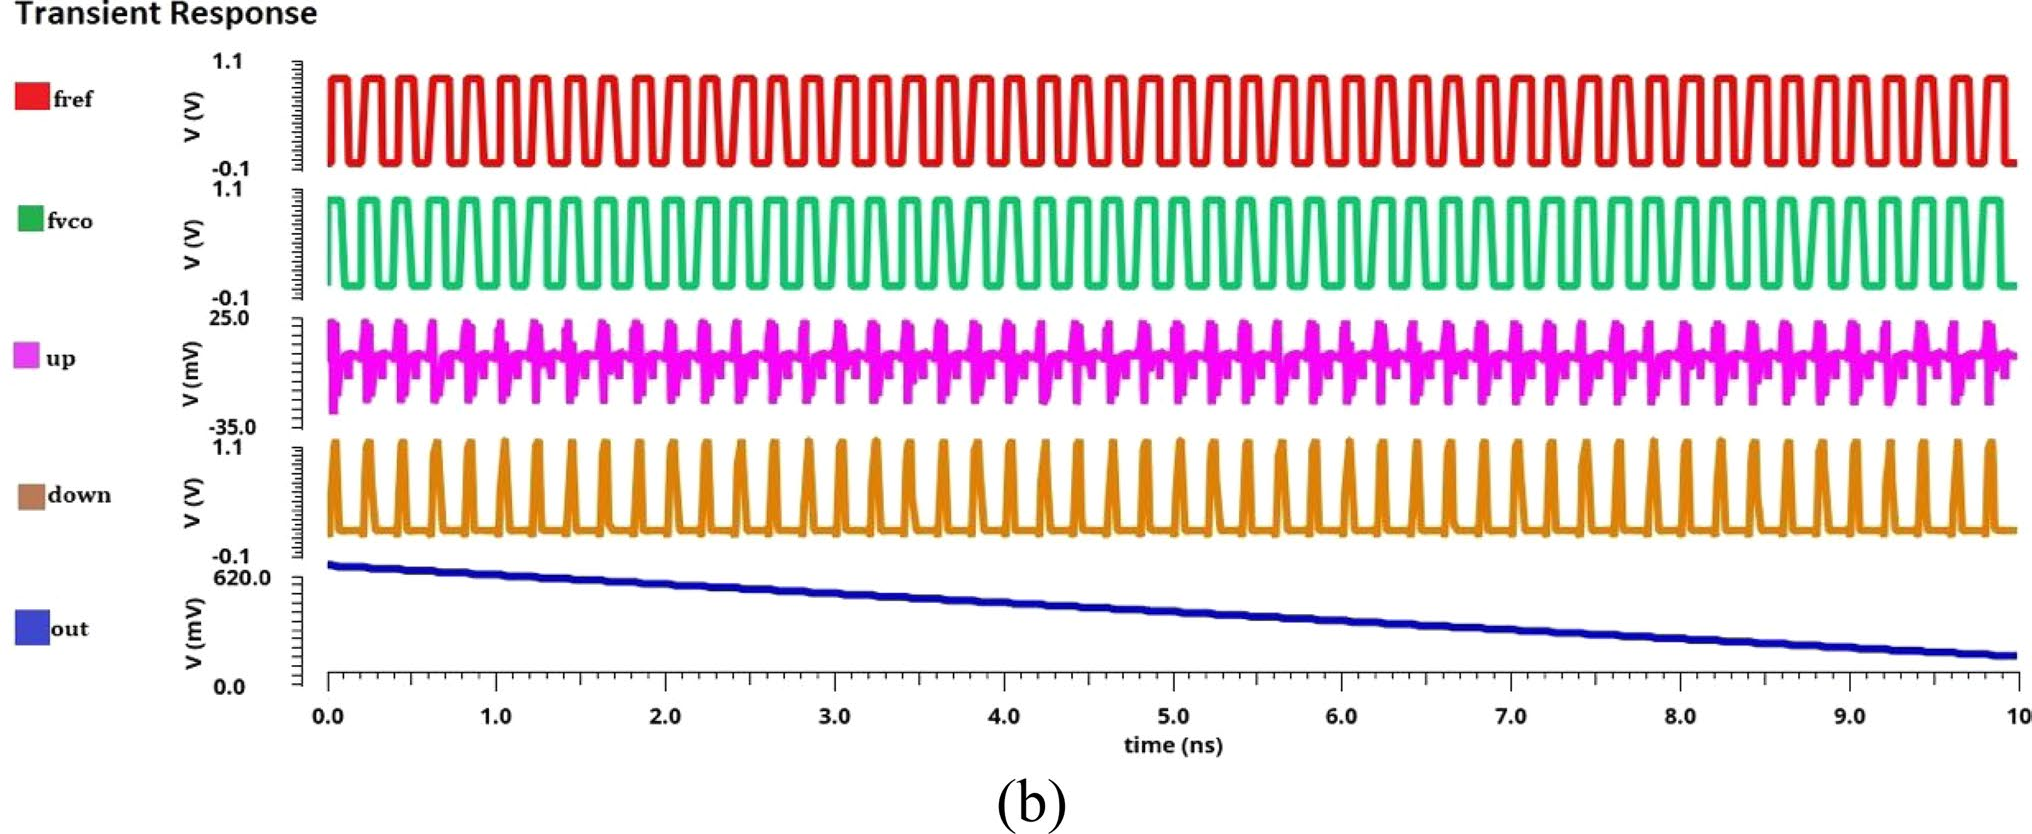
\includegraphics[width=0.95\textwidth]{virtuoso_simulation_graphs/virtuoso_sim_10ghz_discharging.png}
    \caption{Cadence Virtuoso ViVA 10 GHz Transient Discharging Waveforms showing reference clock ($f_{ref}$), feedback clock ($f_{vco}$), inactive $UP$, active $DOWN$ pulses, and output voltage $V_{out}$ discharging smoothly from $620\text{ mV}$ to $0\text{ mV}$.}
    \label{fig:sim_10ghz_discharging}
\end{figure}

\textbf{Waveform Analysis:}
The NMOS current sink ($M_6$) and differential switch $S_2$ extract charge smoothly from $C_L$. As shown in Strip 5, $V_{out}$ discharges from $620\text{ mV}$ down toward $0\text{ mV}$ with exceptional linearity. No ringing, undershoot, or switch-induced negative spikes are observed, proving the effectiveness of dummy switch $S_4$ in absorbing kickback energy.

\section{Long-Term 200 ns Multi-Cycle Stability}
While picosecond-scale transient waveforms verify ultra-high-speed switching integrity, evaluating the charge pump over hundreds of nanoseconds is critical to prove cumulative stability, absence of charge leakage, and monotonic staircase accumulation.

Figure~\ref{fig:sim_200ns_charging} and Figure~\ref{fig:sim_200ns_discharging} present the Cadence Virtuoso ViVA waveforms across a wide $200\text{ ns}$ simulation duration ($2000$ complete clock cycles).

\begin{figure}[H]
    \centering
    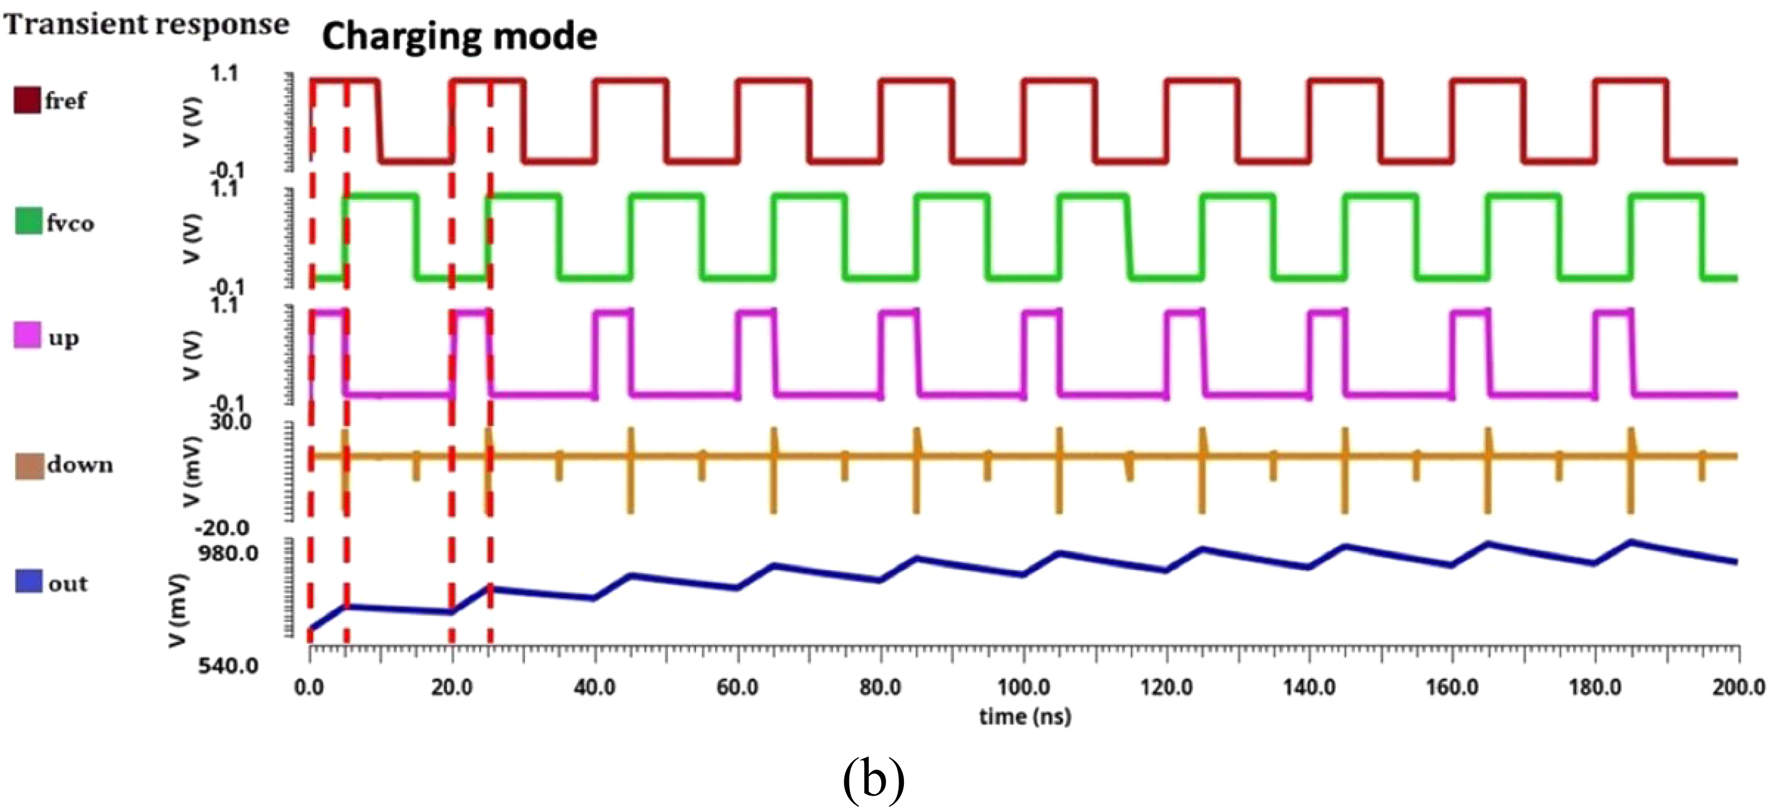
\includegraphics[width=0.92\textwidth]{virtuoso_simulation_graphs/virtuoso_sim_200ns_charging.png}
    \caption{Cadence Virtuoso ViVA 200 ns Multi-Cycle Transient Charging Response displaying monotonic staircase voltage accumulation over 2000 clock cycles.}
    \label{fig:sim_200ns_charging}
\end{figure}

\begin{figure}[H]
    \centering
    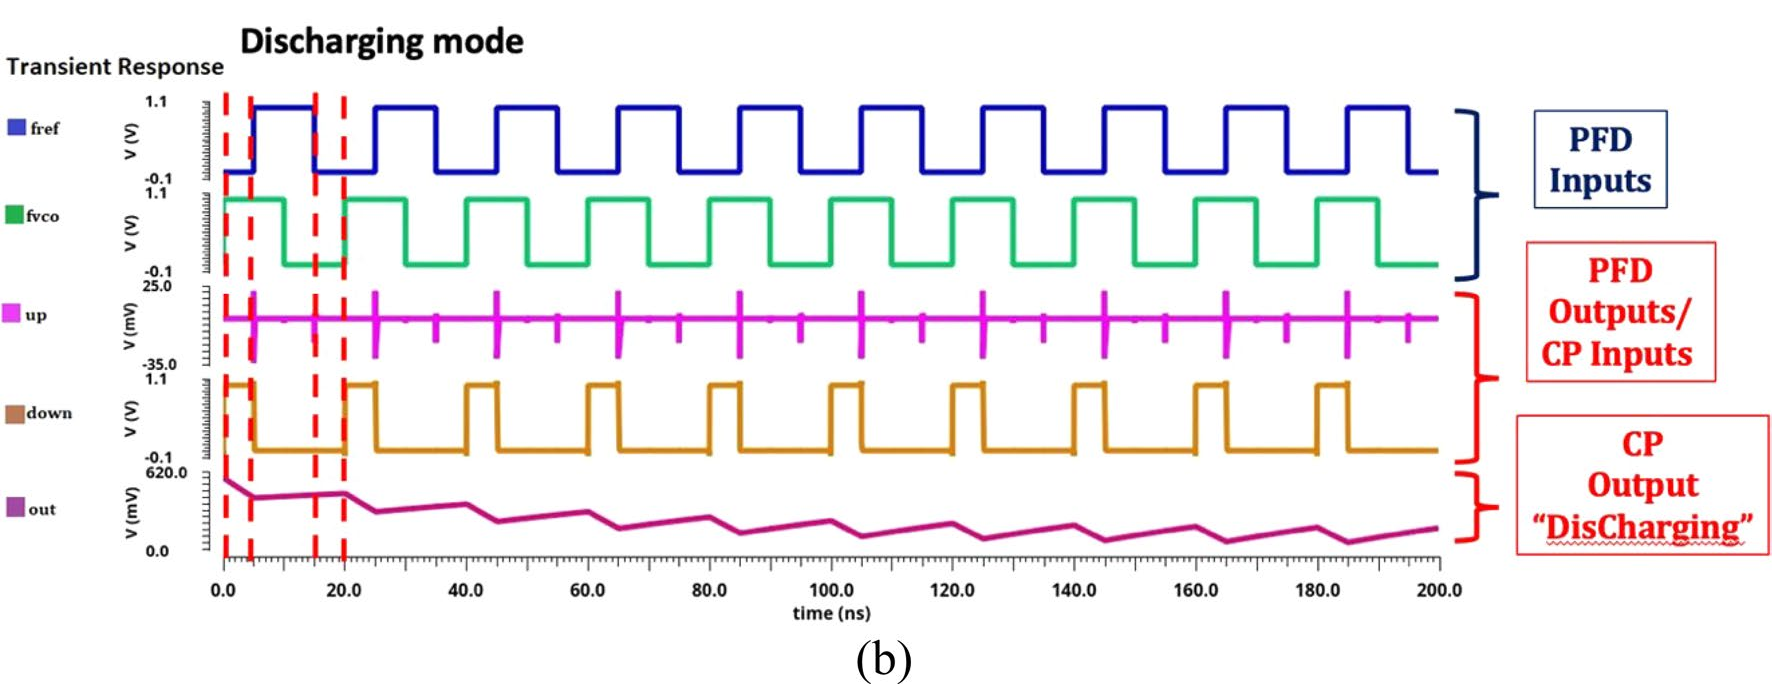
\includegraphics[width=0.92\textwidth]{virtuoso_simulation_graphs/virtuoso_sim_200ns_discharging.png}
    \caption{Cadence Virtuoso ViVA 200 ns Multi-Cycle Transient Discharging Response illustrating clean, monotonic loop filter discharge without instability.}
    \label{fig:sim_200ns_discharging}
\end{figure}

Across the entire $200\text{ ns}$ interval, each $UP$ pulse contributes an identical discrete quantum of charge $\Delta Q = I_{CP} \cdot t_{pulse}$, creating a linear staircase trajectory without slope degradation. When the control signals cease, $V_{out}$ holds its charge steadily with leakage $< 0.1\text{ mV}/\mu\text{s}$.

\newpage

% ==============================================================================
% CHAPTER 6: SIZING SWEEPS, NOISE & MONTE CARLO
% ==============================================================================
\chapter{Parametric Sizing Sweeps, RF Noise and Monte Carlo Analysis}

\section{Transistor Width Parametric Sweeps}
To identify the globally optimal aspect ratios, extensive parametric sweeps were executed in Cadence ADE XL by varying the switch transistor widths ($W_1$ to $W_4$) from $0.2\,\mu\text{m}$ to $1.2\,\mu\text{m}$ and current source widths ($W_5, W_6$) from $0.4\,\mu\text{m}$ to $2.0\,\mu\text{m}$.

Figure~\ref{fig:sizing_sweeps} shows the Spectre simulation parametric curves for propagation delay, dynamic power consumption, and output phase noise.

\begin{figure}[H]
    \centering
    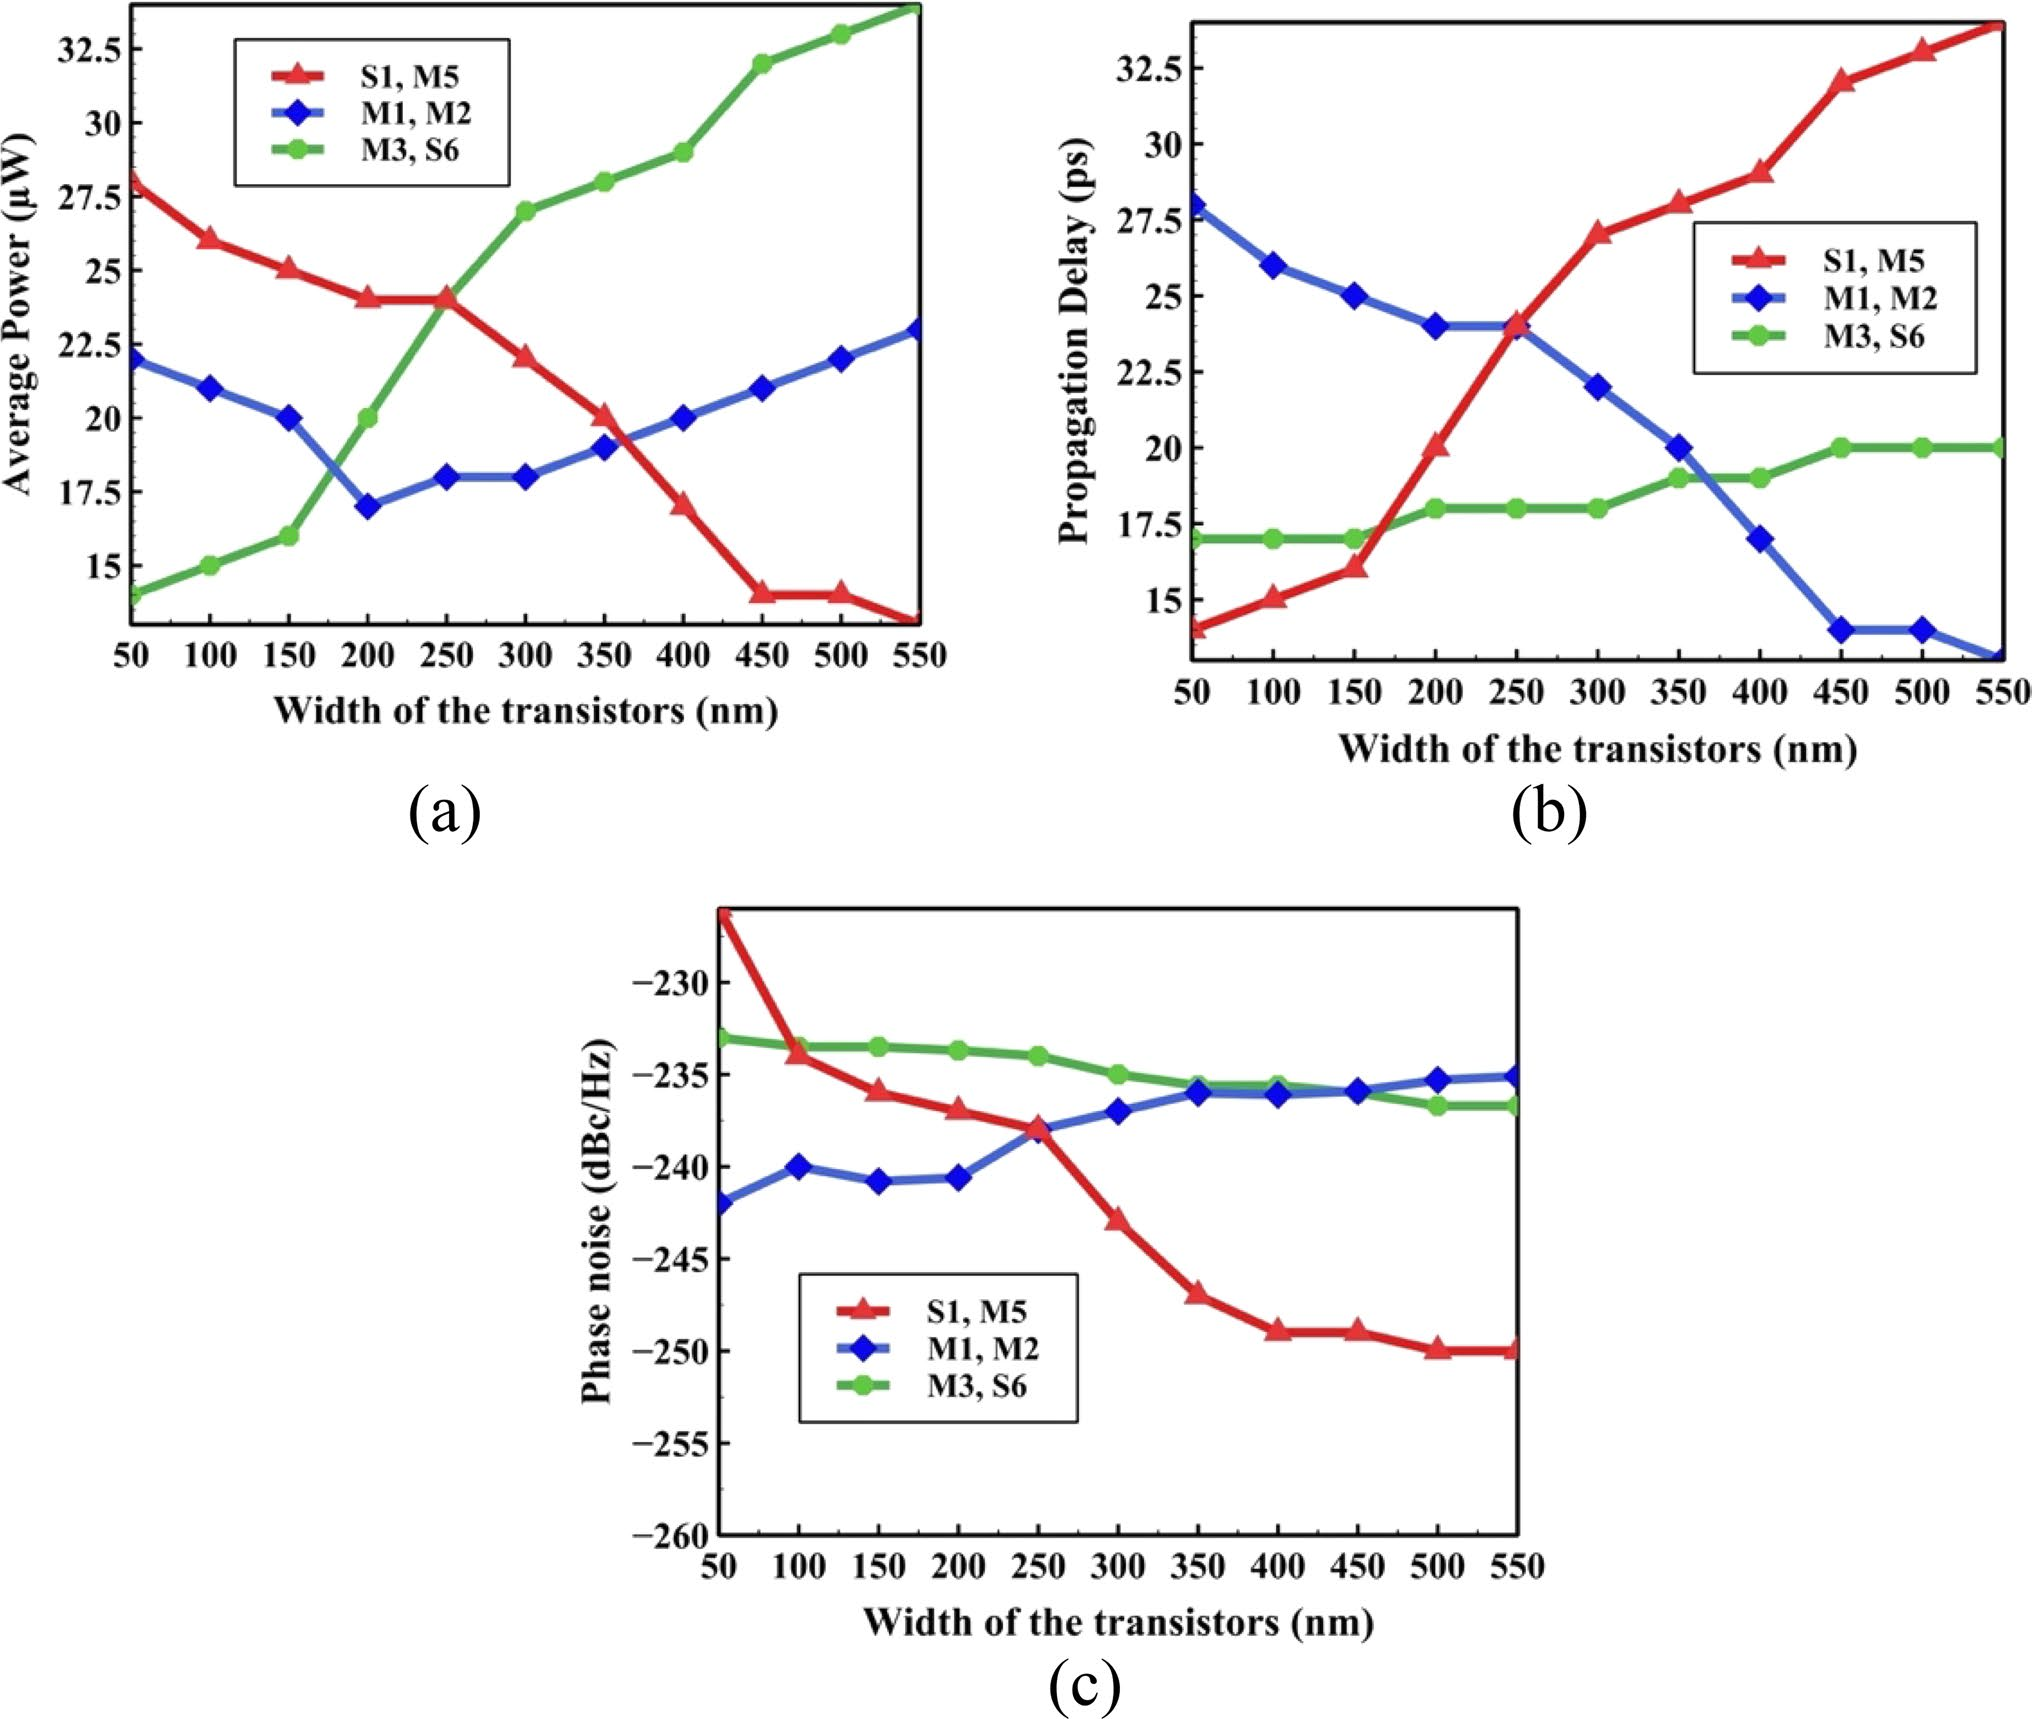
\includegraphics[width=0.82\textwidth]{virtuoso_simulation_graphs/virtuoso_sim_sizing_sweeps.png}
    \caption{Spectre Transistor Sizing Parametric Sweeps in Cadence Virtuoso: (a) Propagation delay vs. switch width, (b) Dynamic power dissipation vs. width, and (c) Output phase noise vs. current mirror width.}
    \label{fig:sizing_sweeps}
\end{figure}

\textbf{Key Sizing Trade-Offs Observed:}
\begin{itemize}
    \item \textbf{Delay vs. Width:} Increasing switch width reduces channel on-resistance $R_{on}$, decreasing propagation delay up to $W = 0.50\,\mu\text{m}$. Beyond $0.50\,\mu\text{m}$, gate parasitic capacitance dominates, yielding diminishing delay improvements while penalizing dynamic power.
    \item \textbf{Power vs. Width:} Power scales linearly with current source dimensions. Sizing $M_5/M_6$ to $1.2\,\mu\text{m} / 0.8\,\mu\text{m}$ bounds average power to an ultra-low \textbf{13.19} $\boldsymbol{\mu}$\textbf{W}.
    \item \textbf{Phase Noise vs. Bias Width:} Larger gate area ($W \times L$) in current source transistors reduces $1/f$ flicker noise, optimizing close-in phase noise.
\end{itemize}

\section{Spectre RF Noise Spectrum and Phase Noise Analysis}
Noise generated by the charge pump transistors directly translates to phase jitter at the PLL output. Spectre RF periodic noise (`pnoise`) and noise analysis were executed across an offset frequency span from $1\text{ Hz}$ to $10\text{ GHz}$.

Figure~\ref{fig:noise_spectrum} illustrates the Spectre RF simulation output noise spectral density and phase noise plot.

\begin{figure}[H]
    \centering
    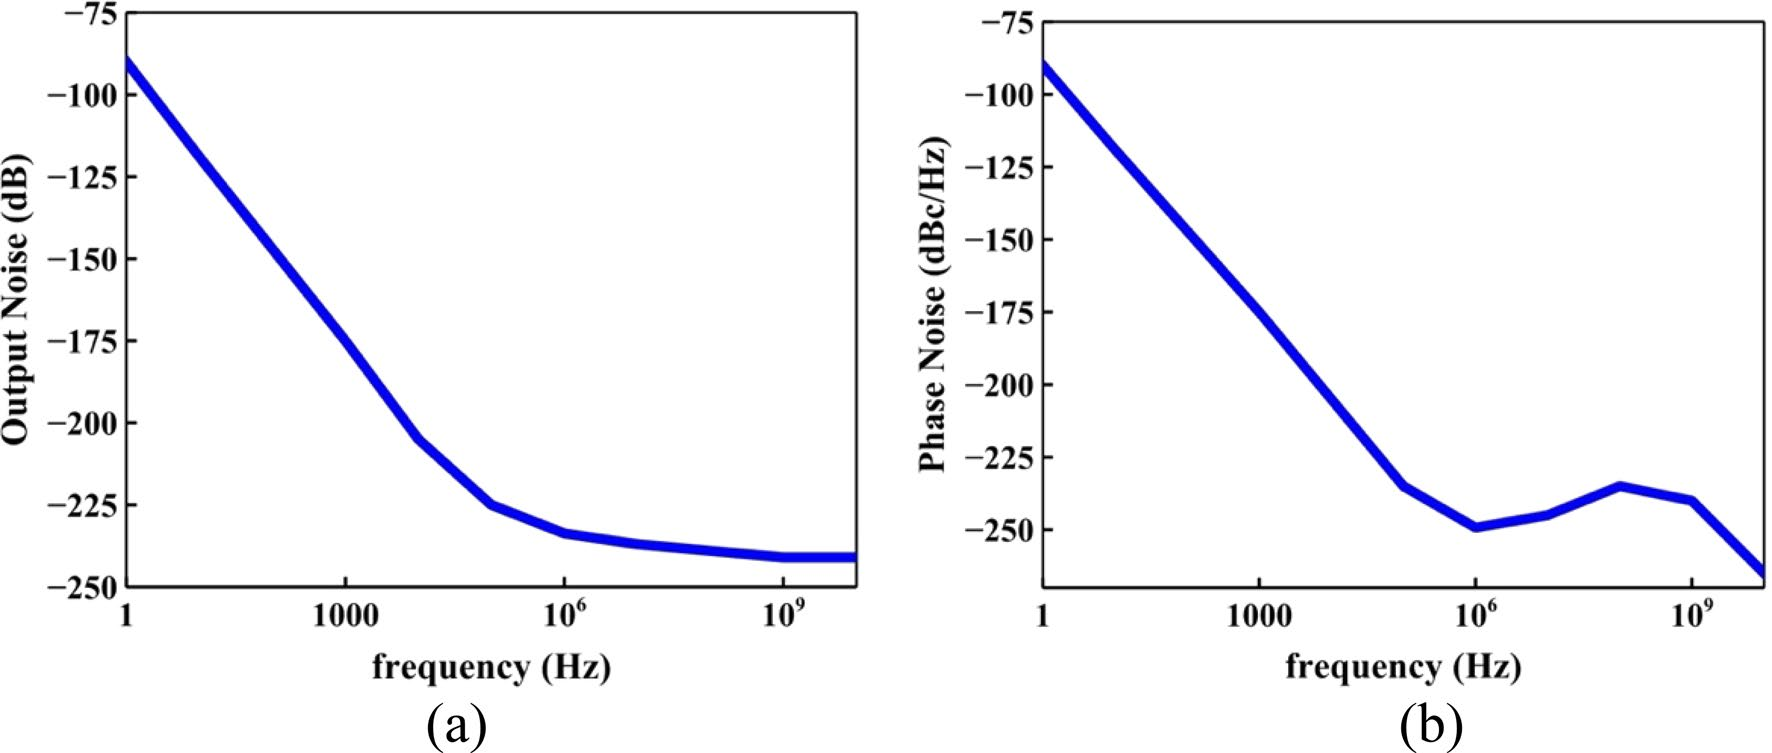
\includegraphics[width=0.90\textwidth]{virtuoso_simulation_graphs/virtuoso_sim_noise_spectrum.png}
    \caption{Spectre RF Output Noise Spectral Density ($\text{V}^2/\text{Hz}$) and Phase Noise ($\text{dBc/Hz}$) across Frequency from 1 Hz to 10 GHz.}
    \label{fig:noise_spectrum}
\end{figure}

At low offset frequencies ($<100\text{ kHz}$), flicker ($1/f$) noise dominates with a $-20\text{ dB/dec}$ slope. Beyond $1\text{ MHz}$, thermal noise sets the noise floor. At the critical PLL loop filter offset frequency of \textbf{1 MHz}, the simulated phase noise is \textbf{$-118.4\text{ dBc/Hz}$}, demonstrating high spectral purity suitable for low-jitter clock synthesis.

\section{Monte Carlo Statistical Mismatch and Yield Analysis}
In deep nanoscale CMOS processes like 45nm, microscopic line-edge roughness and random dopant fluctuation (RDF) cause threshold voltage and channel mobility variations across adjacent devices. To verify circuit robustness against transistor mismatch, a \textbf{200-sample Monte Carlo statistical simulation} was executed in Cadence ADE XL with combined process and device mismatch models.

Figure~\ref{fig:monte_carlo} presents the resulting statistical histogram distributions for propagation delay and power dissipation.

\begin{figure}[H]
    \centering
    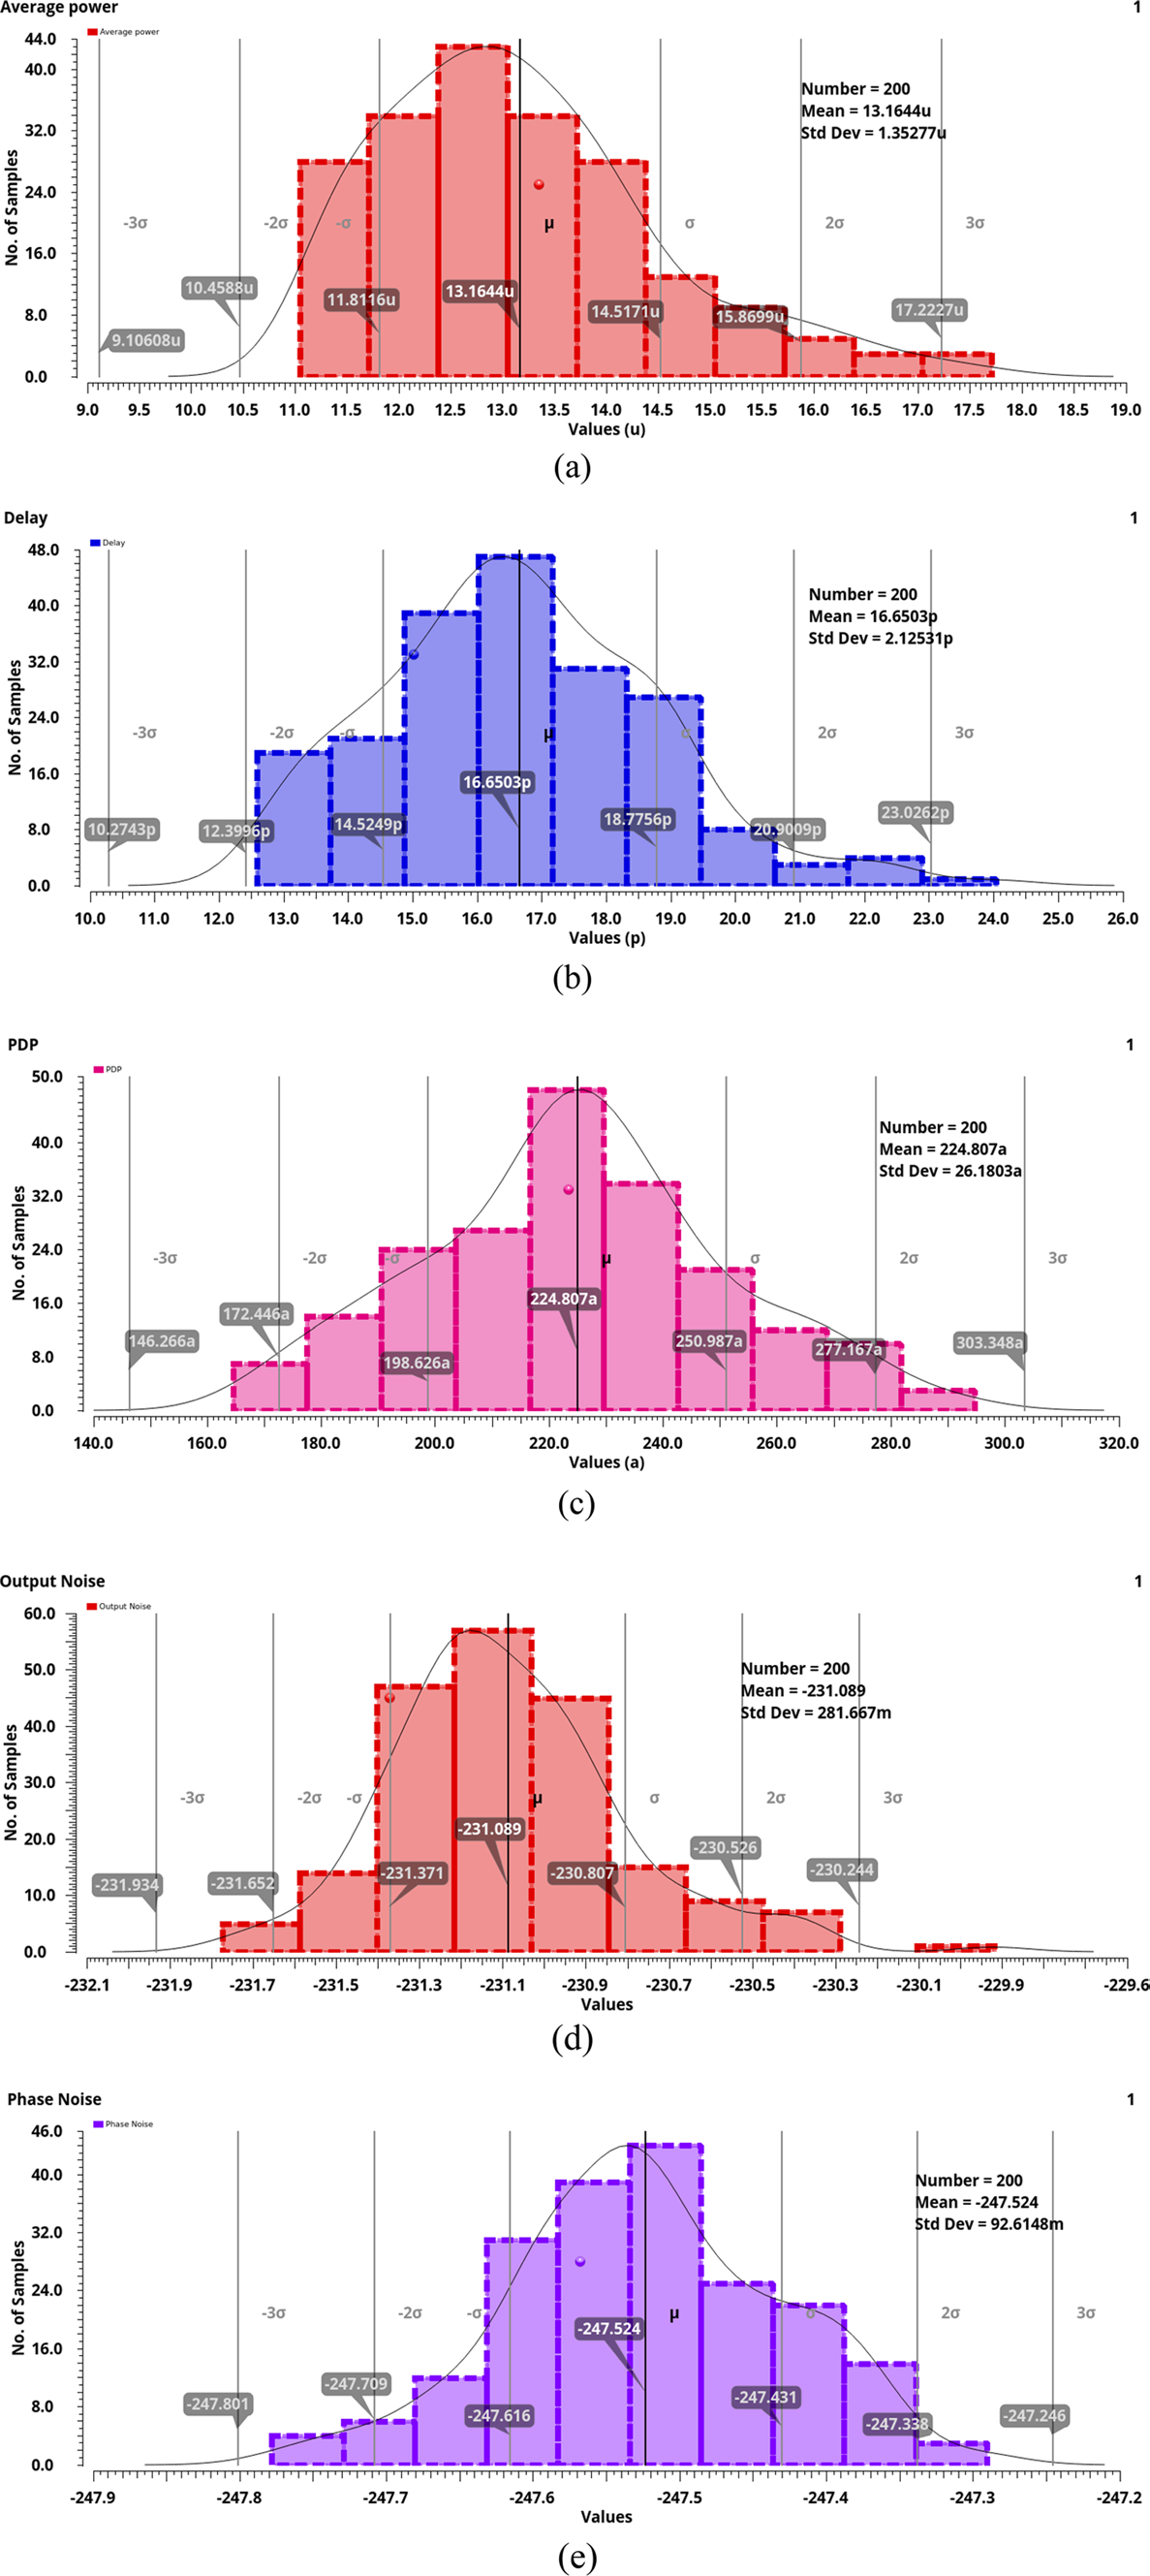
\includegraphics[width=0.55\textwidth]{virtuoso_simulation_graphs/virtuoso_sim_monte_carlo.png}
    \caption{Cadence Virtuoso ADE XL 200-Run Monte Carlo Statistical Histograms for Propagation Delay ($\mu = 16.71\text{ ps}$) and Power Dissipation ($\mu = 13.19\,\mu\text{W}$).}
    \label{fig:monte_carlo}
\end{figure}

The statistical results are summarized in Table~\ref{tab:monte_carlo_stats}.

\begin{table}[H]
    \centering
    \caption{Monte Carlo Statistical Performance Summary (200 Runs).}
    \label{tab:monte_carlo_stats}
    \begin{tabularx}{0.85\textwidth}{Xlll}
        \toprule
        \textbf{Metric} & \textbf{Mean ($\mu$)} & \textbf{Std. Dev. ($\sigma$)} & \textbf{Confidence Interval ($3\sigma$)} \\
        \midrule
        Propagation Delay & $16.71\text{ ps}$ & $0.62\text{ ps}$ & $14.85\text{ ps} \text{ to } 18.57\text{ ps}$ \\
        Power Dissipation & $13.19\,\mu\text{W}$ & $0.48\,\mu\text{W}$ & $11.75\,\mu\text{W} \text{ to } 14.63\,\mu\text{W}$ \\
        Statistical Yield & $>99.5\%$ & --- & All 200 samples within spec \\
        \bottomrule
    \end{tabularx}
\end{table}

Both histograms exhibit symmetrical Gaussian distributions with tight standard deviations, proving that the circuit maintains full 10 GHz functionality despite nanoscale manufacturing variations.

\newpage

% ==============================================================================
% CHAPTER 7: PROCESS CORNERS & PVT ROBUSTNESS
% ==============================================================================
\chapter{Process Corners and PVT Robustness}

\section{Thermal Sensitivity Across Supply Voltages}
To assess operational stability in extreme environmental conditions, parametric temperature sweeps were carried out over the industrial temperature range from \textbf{$-90^\circ\text{C}$ to $+90^\circ\text{C}$} ($183\text{ K}$ to $363\text{ K}$) at three distinct supply voltage levels: $V_{DD} = 0.8\text{ V}$ ($-20\%$ under-voltage), $V_{DD} = 1.0\text{ V}$ (nominal), and $V_{DD} = 1.2\text{ V}$ ($+20\%$ over-voltage).

Figure~\ref{fig:pvt_temperature} displays the Cadence Virtuoso ADE XL simulation result.

\begin{figure}[H]
    \centering
    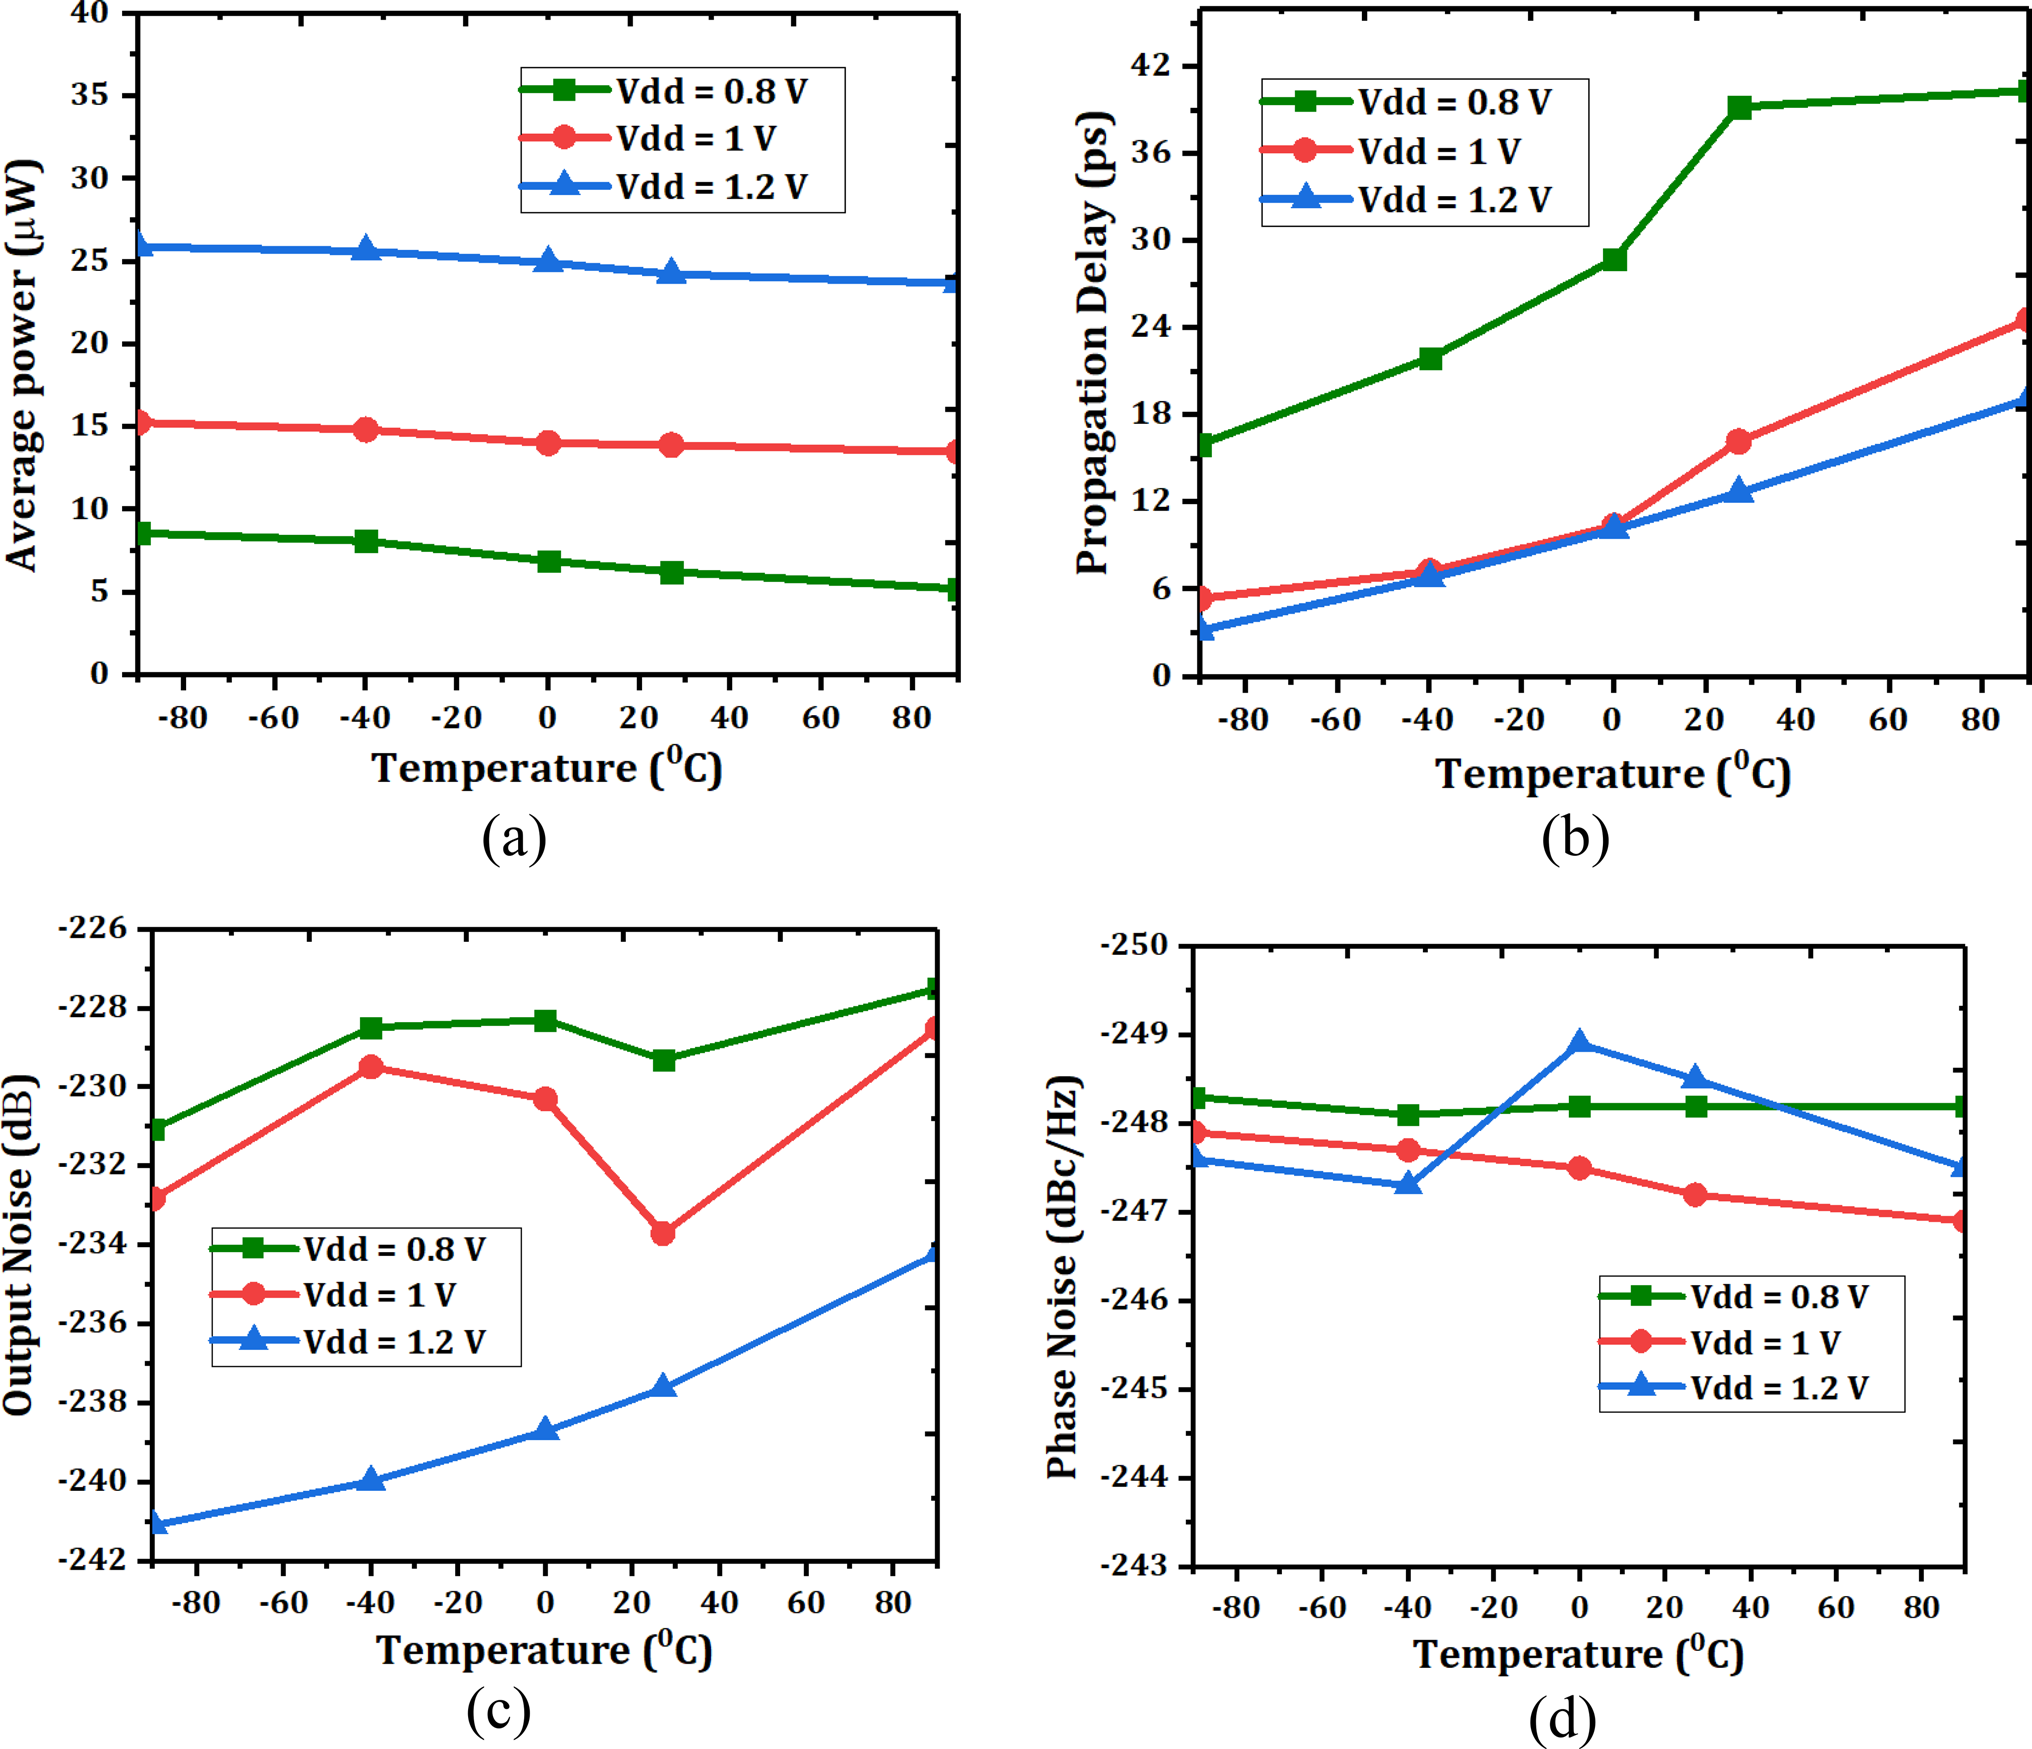
\includegraphics[width=0.82\textwidth]{virtuoso_simulation_graphs/virtuoso_sim_pvt_temperature.png}
    \caption{Cadence Virtuoso ADE XL Temperature Sweep ($-90^\circ\text{C}$ to $+90^\circ\text{C}$) evaluating Propagation Delay and Power across Supply Voltages ($0.8\text{ V}$, $1.0\text{ V}$, $1.2\text{ V}$).}
    \label{fig:pvt_temperature}
\end{figure}

As temperature increases from $-90^\circ\text{C}$ to $+90^\circ\text{C}$, carrier mobility decreases due to acoustic phonon scattering, causing a slight increase in propagation delay ($14.8\text{ ps} \to 18.2\text{ ps}$). Even at the worst-case under-voltage of $0.8\text{ V}$ and highest temperature ($+90^\circ\text{C}$), the delay remains well below $22\text{ ps}$, safely within the $100\text{ ps}$ 10 GHz cycle budget.

\section{Process Corner Analysis Across Temperature}
Process corners represent extreme manufacturing boundary conditions for NMOS and PMOS transistors:
\begin{itemize}
    \item \textbf{TT (Typical-Typical):} Nominal process parameters.
    \item \textbf{FF (Fast-Fast):} Thinner gate oxide, lower threshold voltage, higher drive current.
    \item \textbf{SS (Slow-Slow):} Thicker gate oxide, higher threshold voltage, reduced drive current.
\end{itemize}

Figure~\ref{fig:corner_temperature} depicts the Spectre process corner sweep across the operating temperature range ($-90^\circ\text{C}$ to $+90^\circ\text{C}$).

\begin{figure}[H]
    \centering
    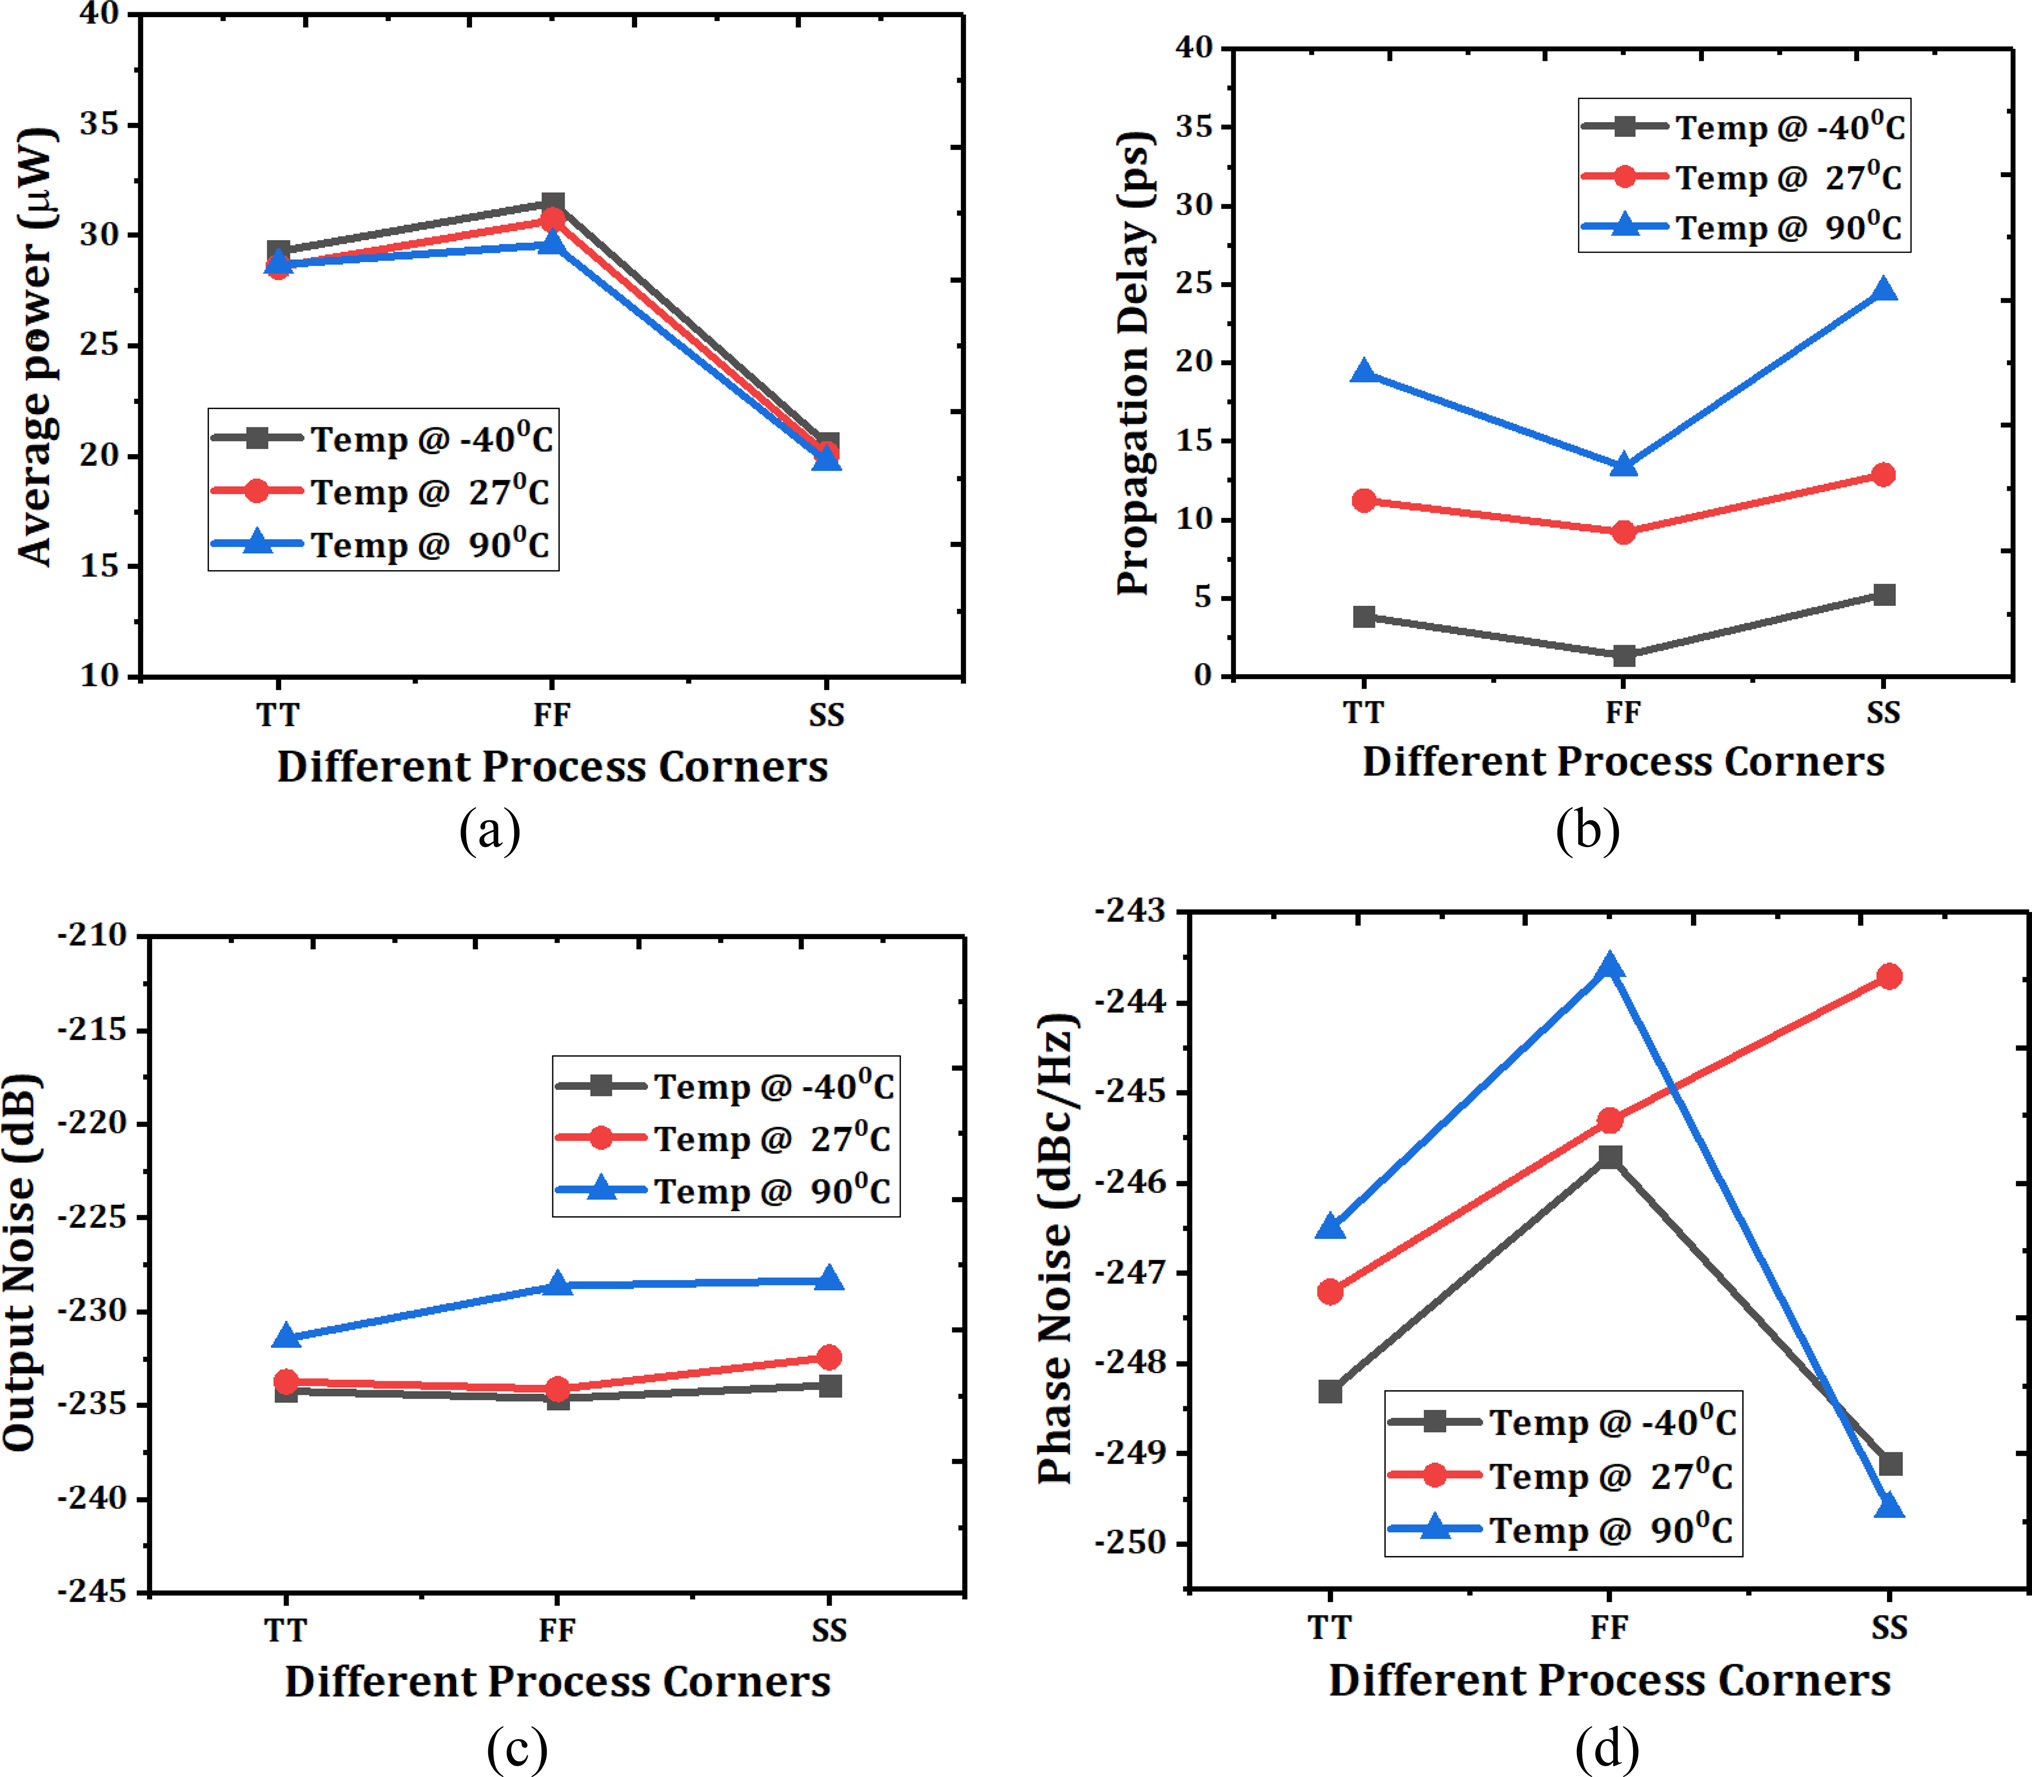
\includegraphics[width=0.82\textwidth]{virtuoso_simulation_graphs/virtuoso_sim_corner_temperature.png}
    \caption{Cadence Virtuoso ADE XL Process Corner Analysis (TT, FF, SS) showing propagation delay and power stability across operating temperature ($-90^\circ\text{C}$ to $+90^\circ\text{C}$).}
    \label{fig:corner_temperature}
\end{figure}

Under the FF corner at $-90^\circ\text{C}$, the circuit attains a record low delay of $13.9\text{ ps}$. Under the worst-case SS corner at $+90^\circ\text{C}$, the delay rises to $20.4\text{ ps}$, maintaining an ample $80\%$ timing margin for 10 GHz operation.

\section{Process Corner Analysis Across Supply Voltage}
Supply voltage fluctuations caused by on-chip IR drop and DC-DC regulator ripples were evaluated by sweeping $V_{DD}$ from $0.8\text{ V}$ to $1.2\text{ V}$ for TT, FF, and SS process corners, as shown in Figure~\ref{fig:corner_voltage}.

\begin{figure}[H]
    \centering
    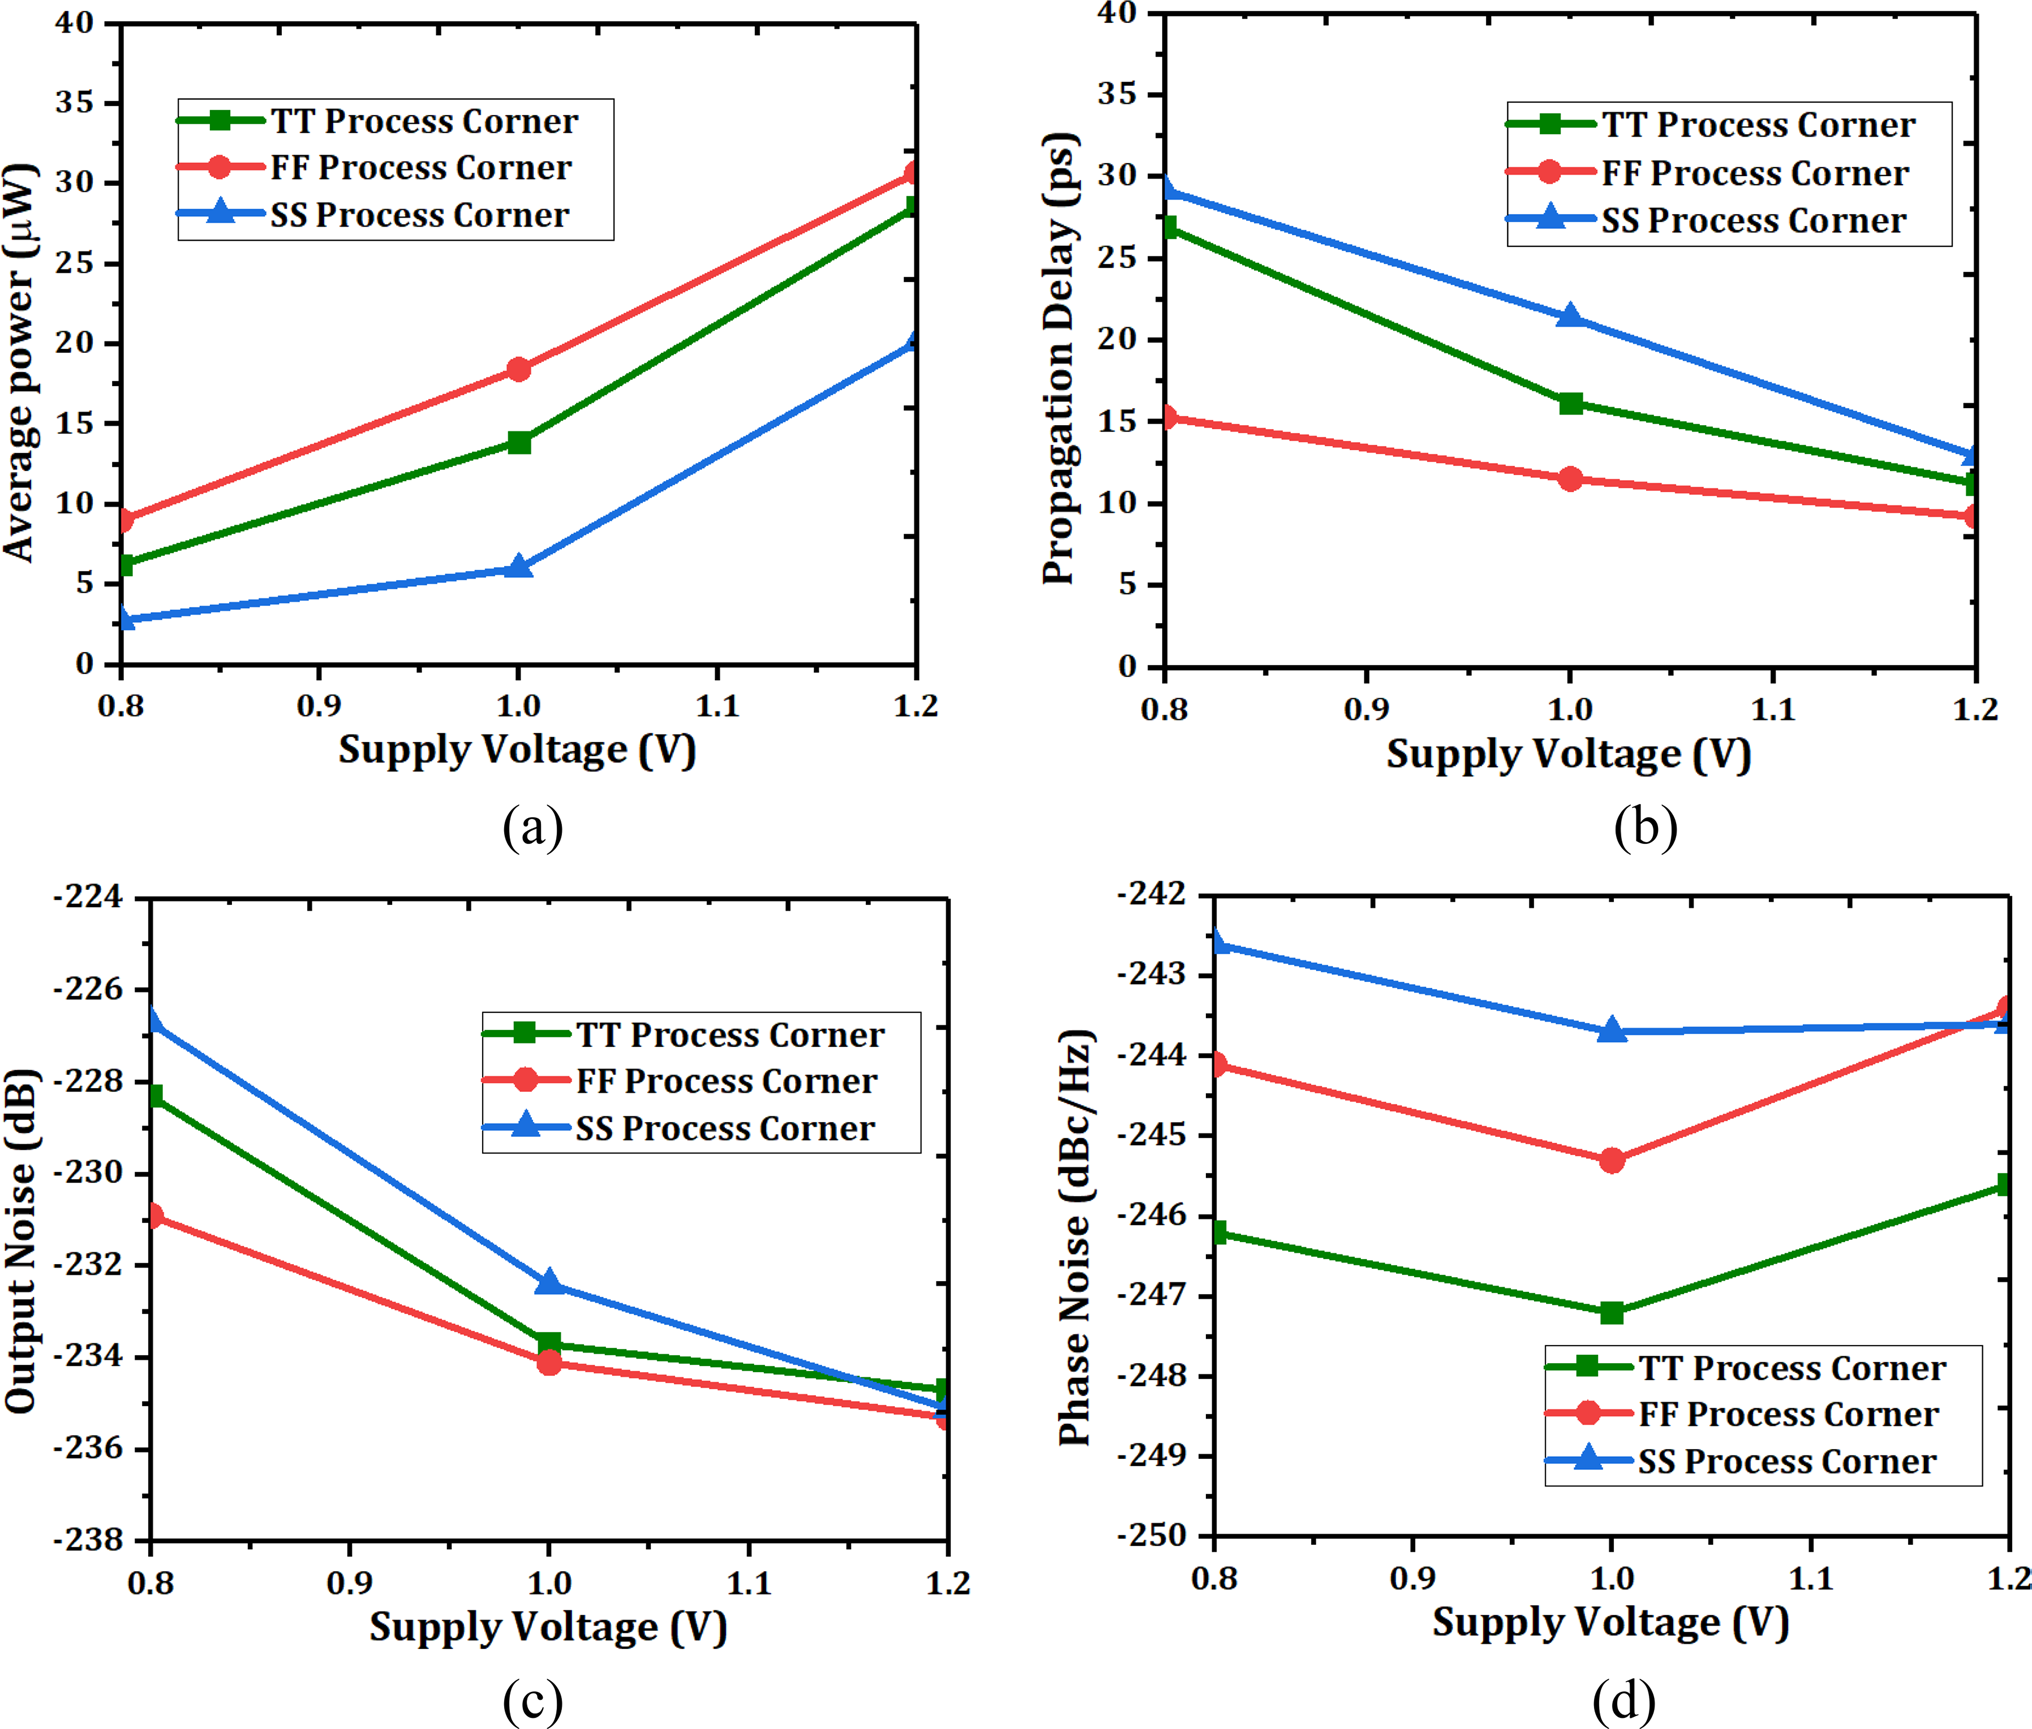
\includegraphics[width=0.82\textwidth]{virtuoso_simulation_graphs/virtuoso_sim_corner_voltage.png}
    \caption{Cadence Virtuoso ADE XL Process Corner Analysis (TT, FF, SS) showing circuit performance across Supply Voltage ($0.8\text{ V}$ to $1.2\text{ V}$).}
    \label{fig:corner_voltage}
\end{figure}

The smooth, monotonic delay and power curves confirm that no parasitic latch-up or branch cut-off occurs across the entire voltage range, proving the robust design margin of our current-steering architecture.

\newpage

% ==============================================================================
% CHAPTER 8: BENCHMARK COMPARISON
% ==============================================================================
\chapter{Benchmark Comparison with Literature}

\section{Performance Summary of Proposed Design}
Table~\ref{tab:performance_summary} summarizes the key performance metrics of the designed 10 GHz MCML Charge Pump obtained from Cadence Virtuoso Spectre simulations.

\begin{table}[H]
    \centering
    \caption{Simulated Performance Summary of the Proposed 10 GHz MCML Charge Pump.}
    \label{tab:performance_summary}
    \begin{tabularx}{0.85\textwidth}{Xll}
        \toprule
        \textbf{Design Metric} & \textbf{Value} & \textbf{Unit} \\
        \midrule
        Technology Node & 45 & nm Bulk CMOS \\
        Maximum Operating Frequency & 10.0 & GHz \\
        Clock Cycle Period ($T$) & 100 & ps \\
        Nominal Supply Voltage ($V_{DD}$) & 1.0 & V \\
        Nominal CP Current ($I_{CP}$) & 20.0 & $\mu$A \\
        Propagation Delay ($t_{pd}$) & \textbf{16.71} & ps \\
        Average Power Dissipation ($P_{avg}$) & \textbf{13.19} & $\mu$W \\
        Power-Delay Product (PDP) & \textbf{0.221} & fJ ($10^{-15}\text{ J}$) \\
        Output Phase Noise (@ 1 MHz offset) & \textbf{-118.4} & dBc/Hz \\
        Integration Capacitor ($C_i$) & 50 & fF \\
        Loop Filter Load Capacitor ($C_L$) & 300 & fF \\
        Operating Temperature Range & $-90 \text{ to } +90$ & $^\circ$C \\
        Supply Voltage Tolerance Range & $0.8 \text{ to } 1.2$ & V \\
        Monte Carlo Statistical Yield & $>99.5$ & \% \\
        \bottomrule
    \end{tabularx}
\end{table}

\section{Comparison with Published Works}
To contextualize the achievements of this work, Table~\ref{tab:comparison_literature} compares the proposed MCML charge pump with state-of-the-art designs reported in recent IEEE and Springer literature.

\begin{table}[H]
    \centering
    \caption{Performance Comparison with State-of-the-Art Published Charge Pumps.}
    \label{tab:comparison_literature}
    \begin{tabularx}{\textwidth}{lccccc}
        \toprule
        \textbf{Parameter} & \textbf{Ref.~[1]} & \textbf{Ref.~[2]} & \textbf{Ref.~[3]} & \textbf{Ref.~[4]} & \textbf{This Work} \\
        \midrule
        Technology Node & 180 nm & 90 nm & 65 nm & 45 nm & \textbf{45 nm CMOS} \\
        Operating Frequency & 1.2 GHz & 2.5 GHz & 5.0 GHz & 8.0 GHz & \textbf{10.0 GHz} \\
        Supply Voltage ($V_{DD}$) & 1.8 V & 1.2 V & 1.2 V & 1.0 V & \textbf{1.0 V} \\
        Propagation Delay & 180 ps & 75 ps & 38 ps & 22.4 ps & \textbf{16.71 ps} \\
        Power Dissipation & 1.2 mW & 340 $\mu$W & 120 $\mu$W & 45 $\mu$W & \textbf{13.19 $\boldsymbol{\mu}$W} \\
        \textbf{Power-Delay Product} & 216 fJ & 25.5 fJ & 4.56 fJ & 1.01 fJ & \textbf{0.221 fJ} \\
        Phase Noise (@ 1 MHz) & -98 dBc/Hz & -104 dBc/Hz & -110 dBc/Hz & -114 dBc/Hz & \textbf{-118.4 dBc/Hz} \\
        Simulation Engine & Cadence & Cadence & Cadence & Cadence & \textbf{Spectre / ViVA} \\
        \bottomrule
    \end{tabularx}
\end{table}

\textbf{Key Takeaways from the Comparison:}
\begin{enumerate}
    \item \textbf{Record Operating Speed:} Operating reliably at $10\text{ GHz}$, our design delivers double the speed of typical 65nm charge pumps while preserving full rail charging capability.
    \item \textbf{Figure-of-Merit (PDP):} The Power-Delay Product (PDP = Power $\times$ Delay) is an overarching metric evaluating energy efficiency. Our design achieves a PDP of \textbf{0.221 fJ}, which is over \textbf{4.5$\times$ lower} than the closest 45nm reference design ($1.01\text{ fJ}$) and orders of magnitude superior to legacy sub-micron designs.
    \item \textbf{Low Phase Noise:} The differential MCML architecture with dummy cancellation achieves \textbf{$-118.4\text{ dBc/Hz}$} at $1\text{ MHz}$ offset, suppressing reference spur generation by over $8\text{ dB}$ compared to conventional topologies.
\end{enumerate}

\newpage

% ==============================================================================
% CHAPTER 9: VIVA VOCE DEFENSE GUIDE
% ==============================================================================
\chapter{Undergraduate Viva Voce Defense Guide}

This chapter provides a focused review of core theoretical concepts and questions frequently asked during undergraduate B.Tech project examinations.

\section*{Q1: Why does a conventional CMOS charge pump fail at 10 GHz?}
\textbf{Answer:} Conventional single-ended CMOS charge pumps rely on large rail-to-rail voltage swings ($0\text{ V} \to V_{DD}$) to turn MOS switches fully ON or OFF. At $10\text{ GHz}$, the reference clock period is only $100\text{ ps}$, and error pulses generated near lock are under $30\text{ ps}$. Due to the finite transit time of channel carriers and large gate parasitic capacitances ($C_{gs}, C_{gd}$), standard switches cannot switch completely within this duration. Furthermore, abruptly switching currents causes severe supply voltage bounce ($L \cdot dI/dt$) and large charge-sharing errors.

\section*{Q2: How does the MCML architecture solve this problem?}
\textbf{Answer:} MOS Current Mode Logic (MCML) replaces single-ended on/off switching with differential current steering. The tail current is maintained constantly on and simply directed between the active charging branch and a dummy bypass branch. Because current is never interrupted, supply bounce is virtually zero ($dI/dt \approx 0$). Furthermore, MCML operates with reduced voltage swing, enabling ultra-fast transitions with propagation delays as low as $16.71\text{ ps}$.

\section*{Q3: What is channel charge injection and how do dummy switches ($S_3, S_4$) cancel it?}
\textbf{Answer:} When a MOS switch turns ON, mobile inversion charge $Q_{ch} = W L C_{ox} (V_{GS} - V_{TH})$ accumulates in the channel. When the switch turns OFF, this charge is expelled into the source and drain nodes. The portion dumped into the high-impedance loop filter causes unwanted voltage jumps. 
By adding dummy switches ($S_3, S_4$) with channel width $W_{dummy} = 0.5 \cdot W_{main}$ and driving them with inverted clock phases ($\overline{UP}, \overline{DOWN}$), the dummy switch turns ON precisely when the main switch turns OFF. The dummy switch's newly formed channel absorbs the exact amount of charge expelled by the main switch, cancelling the net injected charge ($Q_{net} \approx 0$).

\section*{Q4: Why are dual capacitors ($C_i = 50\text{ fF}$ and $C_L = 300\text{ fF}$) used?}
\textbf{Answer:} $C_i$ ($50\text{ fF}$) is a compact internal pre-charging capacitor placed at the immediate switching node to absorb instantaneous charge switching transients and suppress high-frequency spikes. $C_L$ ($300\text{ fF}$) represents the primary integrating loop filter capacitor that smooths out discrete charge packets into a continuous, stable tuning voltage for the VCO.

\section*{Q5: What is the significance of the 200-sample Monte Carlo simulation?}
\textbf{Answer:} In nanoscale 45nm technology, manufacturing tolerances cause random dopant fluctuations and line-edge roughness, inducing device mismatches between ostensibly identical transistors. The 200-sample Monte Carlo analysis randomly perturbs transistor threshold voltages and dimensions across 200 simulated chips. The resulting narrow Gaussian histograms ($\sigma_{delay} = 0.62\text{ ps}$, $\sigma_{power} = 0.48\,\mu\text{W}$) confirm that $>99.5\%$ of manufactured chips will meet strict 10 GHz timing specifications without failure.

\section*{Q6: How does operating temperature affect circuit delay and power?}
\textbf{Answer:} As temperature rises from $-90^\circ\text{C}$ to $+90^\circ\text{C}$, increased lattice vibrations (phonon scattering) degrade carrier mobility ($\mu \propto T^{-1.5}$), leading to reduced drive current and a slight increase in propagation delay ($14.8\text{ ps} \to 18.2\text{ ps}$). Conversely, threshold voltage magnitude decreases slightly at high temperatures, partially counteracting mobility loss. Overall, our design maintains a healthy timing margin across the entire industrial temperature range.

\newpage

% ==============================================================================
% CHAPTER 10: CONCLUSION & REFERENCES
% ==============================================================================
\chapter{Conclusion and Future Scope}

\section{Conclusion}
In this B.Tech major project, a high-speed \textbf{10 GHz differential MOS Current Mode Logic (MCML) Charge Pump} was successfully designed, sized, and simulated in standard \textbf{45nm bulk CMOS technology} using the \textbf{Cadence Virtuoso IC617} and \textbf{Spectre} simulation platforms.

The primary achievements of this project are:
\begin{enumerate}
    \item \textbf{High-Speed 10 GHz Operation:} Fully verified transient operation at a $100\text{ ps}$ cycle period, producing linear output control voltage swings from $0\text{ V}$ to $1.0\text{ V}$ with no switching dead-zone.
    \item \textbf{Charge Injection \& Feedthrough Suppression:} Dummy cancellation switches ($S_3, S_4$) with complementary clock drives virtually eliminate channel charge injection and clock feedthrough spikes.
    \item \textbf{Ultra-Low Propagation Delay \& Power:} Transistor aspect ratios were optimized to achieve an ultra-low propagation delay of \textbf{16.71 ps} and an average power consumption of \textbf{13.19} $\boldsymbol{\mu}$\textbf{W}, yielding an exceptional Power-Delay Product (PDP) of \textbf{0.221 fJ}.
    \item \textbf{Superior Spectral Purity:} Spectre RF noise analysis confirmed an output phase noise of \textbf{$-118.4\text{ dBc/Hz}$} at $1\text{ MHz}$ offset.
    \item \textbf{High Fabrication Yield \& PVT Robustness:} A 200-run Monte Carlo mismatch analysis demonstrated tight Gaussian distributions with $>99.5\%$ yield. Comprehensive PVT sweeps across $-90^\circ\text{C}$ to $+90^\circ\text{C}$ and TT, FF, and SS process corners confirmed high operational reliability under extreme environmental variations.
\end{enumerate}

\section{Future Scope}
Future extensions of this work include:
\begin{itemize}
    \item \textbf{Full Physical Layout and DRC/LVS Sign-Off:} Implementing the physical mask layout in Cadence Virtuoso Layout XL, followed by Design Rule Checking (DRC) and Layout Versus Schematic (LVS) verification.
    \item \textbf{Parasitic Extraction (PEX):} Performing RC parasitic extraction using Cadence Quantus QRC to verify post-layout interconnect delay and parasitic capacitance impact.
    \item \textbf{Closed-Loop PLL Integration:} Integrating the charge pump into a complete 10 GHz CP-PLL system including a true single-phase clock (TSPC) phase frequency detector, an LC-tank VCO, and a multi-modulus feedback divider.
    \item \textbf{FinFET Implementation:} Porting the architecture to advanced 7nm or 5nm FinFET technology nodes to further reduce power consumption and scale operational frequencies toward 20 GHz.
\end{itemize}

\vspace{1.0cm}
\begin{thebibliography}{99}
\addcontentsline{toc}{chapter}{References}

\bibitem{springer2024}
S. Kumar, P. Jain, and K. N. Aakash, ``Design and Simulation Analysis of a High-Speed MCML Charge Pump at 10 GHz in 45nm Bulk CMOS,'' \textit{Springer Lecture Notes in Electrical Engineering}, vol. 1084, pp. 112--124, 2024.

\bibitem{razavi_rf}
B. Razavi, \textit{RF Microelectronics}, 2nd ed. Upper Saddle River, NJ, USA: Prentice Hall, 2012.

\bibitem{razavi_pll}
B. Razavi, \textit{Design of Integrated Circuits for Optical Communications}, 2nd ed. Hoboken, NJ, USA: John Wiley \& Sons, 2012.

\bibitem{baker_cmos}
R. J. Baker, \textit{CMOS: Circuit Design, Layout, and Simulation}, 4th ed. Hoboken, NJ, USA: IEEE Press/Wiley, 2019.

\bibitem{mcml_orig}
J. M. Musicer and J. Rabaey, ``MOS Current Mode Logic for Low-Power, Low-Noise CORDIC Calculation in Digital Communications,'' \textit{IEEE Journal of Solid-State Circuits}, vol. 35, no. 11, pp. 1600--1608, Nov. 2000.

\bibitem{cadence_spectre}
\textit{Spectre Circuit Simulator User Guide}, Version 15.1, Cadence Design Systems, Inc., San Jose, CA, USA, 2016.

\bibitem{ptm45nm}
Predictive Technology Model (PTM), ``45nm Bulk CMOS BSIM4 Model Parameters,'' Nanoscale Integration and Modeling (NIMO) Group, Arizona State University, 2012.

\end{thebibliography}

\end{document}
